\documentclass[twoside]{book}

% Packages required by doxygen
\usepackage{fixltx2e}
\usepackage{calc}
\usepackage{doxygen}
\usepackage[export]{adjustbox} % also loads graphicx
\usepackage{graphicx}
\usepackage[utf8]{inputenc}
\usepackage{makeidx}
\usepackage{multicol}
\usepackage{multirow}
\PassOptionsToPackage{warn}{textcomp}
\usepackage{textcomp}
\usepackage[nointegrals]{wasysym}
\usepackage[table]{xcolor}

% Font selection
\usepackage[T1]{fontenc}
\usepackage[scaled=.90]{helvet}
\usepackage{courier}
\usepackage{amssymb}
\usepackage{sectsty}
\renewcommand{\familydefault}{\sfdefault}
\allsectionsfont{%
  \fontseries{bc}\selectfont%
  \color{darkgray}%
}
\renewcommand{\DoxyLabelFont}{%
  \fontseries{bc}\selectfont%
  \color{darkgray}%
}
\newcommand{\+}{\discretionary{\mbox{\scriptsize$\hookleftarrow$}}{}{}}

% Page & text layout
\usepackage{geometry}
\geometry{%
  a4paper,%
  top=2.5cm,%
  bottom=2.5cm,%
  left=2.5cm,%
  right=2.5cm%
}
\tolerance=750
\hfuzz=15pt
\hbadness=750
\setlength{\emergencystretch}{15pt}
\setlength{\parindent}{0cm}
\setlength{\parskip}{3ex plus 2ex minus 2ex}
\makeatletter
\renewcommand{\paragraph}{%
  \@startsection{paragraph}{4}{0ex}{-1.0ex}{1.0ex}{%
    \normalfont\normalsize\bfseries\SS@parafont%
  }%
}
\renewcommand{\subparagraph}{%
  \@startsection{subparagraph}{5}{0ex}{-1.0ex}{1.0ex}{%
    \normalfont\normalsize\bfseries\SS@subparafont%
  }%
}
\makeatother

% Headers & footers
\usepackage{fancyhdr}
\pagestyle{fancyplain}
\fancyhead[LE]{\fancyplain{}{\bfseries\thepage}}
\fancyhead[CE]{\fancyplain{}{}}
\fancyhead[RE]{\fancyplain{}{\bfseries\leftmark}}
\fancyhead[LO]{\fancyplain{}{\bfseries\rightmark}}
\fancyhead[CO]{\fancyplain{}{}}
\fancyhead[RO]{\fancyplain{}{\bfseries\thepage}}
\fancyfoot[LE]{\fancyplain{}{}}
\fancyfoot[CE]{\fancyplain{}{}}
\fancyfoot[RE]{\fancyplain{}{\bfseries\scriptsize Generated by Doxygen }}
\fancyfoot[LO]{\fancyplain{}{\bfseries\scriptsize Generated by Doxygen }}
\fancyfoot[CO]{\fancyplain{}{}}
\fancyfoot[RO]{\fancyplain{}{}}
\renewcommand{\footrulewidth}{0.4pt}
\renewcommand{\chaptermark}[1]{%
  \markboth{#1}{}%
}
\renewcommand{\sectionmark}[1]{%
  \markright{\thesection\ #1}%
}

% Indices & bibliography
\usepackage{natbib}
\usepackage[titles]{tocloft}
\setcounter{tocdepth}{3}
\setcounter{secnumdepth}{5}
\makeindex

% Hyperlinks (required, but should be loaded last)
\usepackage{ifpdf}
\ifpdf
  \usepackage[pdftex,pagebackref=true]{hyperref}
\else
  \usepackage[ps2pdf,pagebackref=true]{hyperref}
\fi
\hypersetup{%
  colorlinks=true,%
  linkcolor=blue,%
  citecolor=blue,%
  unicode%
}

% Custom commands
\newcommand{\clearemptydoublepage}{%
  \newpage{\pagestyle{empty}\cleardoublepage}%
}

\usepackage{caption}
\captionsetup{labelsep=space,justification=centering,font={bf},singlelinecheck=off,skip=4pt,position=top}

%===== C O N T E N T S =====

\begin{document}

% Titlepage & ToC
\hypersetup{pageanchor=false,
             bookmarksnumbered=true,
             pdfencoding=unicode
            }
\pagenumbering{alph}
\begin{titlepage}
\vspace*{7cm}
\begin{center}%
{\Large Gopher Server }\\
\vspace*{1cm}
{\large Generated by Doxygen 1.8.13}\\
\end{center}
\end{titlepage}
\clearemptydoublepage
\pagenumbering{roman}
\tableofcontents
\clearemptydoublepage
\pagenumbering{arabic}
\hypersetup{pageanchor=true}

%--- Begin generated contents ---
\chapter{Class Index}
\section{Class List}
Here are the classes, structs, unions and interfaces with brief descriptions\+:\begin{DoxyCompactList}
\item\contentsline{section}{\hyperlink{structfile__mapping__t}{file\+\_\+mapping\+\_\+t} }{\pageref{structfile__mapping__t}}{}
\item\contentsline{section}{\hyperlink{structlogger__t}{logger\+\_\+t} \\*An object }{\pageref{structlogger__t}}{}
\item\contentsline{section}{\hyperlink{structsend__args__t}{send\+\_\+args\+\_\+t} }{\pageref{structsend__args__t}}{}
\item\contentsline{section}{\hyperlink{structserver__t}{server\+\_\+t} }{\pageref{structserver__t}}{}
\item\contentsline{section}{\hyperlink{structserver__thread__args__t}{server\+\_\+thread\+\_\+args\+\_\+t} }{\pageref{structserver__thread__args__t}}{}
\end{DoxyCompactList}

\chapter{File Index}
\section{File List}
Here is a list of all files with brief descriptions\+:\begin{DoxyCompactList}
\item\contentsline{section}{headers/\hyperlink{constants_8h}{constants.\+h} }{\pageref{constants_8h}}{}
\item\contentsline{section}{headers/\hyperlink{datatypes_8h}{datatypes.\+h} }{\pageref{datatypes_8h}}{}
\item\contentsline{section}{headers/\hyperlink{log_8h}{log.\+h} }{\pageref{log_8h}}{}
\item\contentsline{section}{headers/\hyperlink{logger_8h}{logger.\+h} }{\pageref{logger_8h}}{}
\item\contentsline{section}{headers/\hyperlink{platform_8h}{platform.\+h} }{\pageref{platform_8h}}{}
\item\contentsline{section}{headers/\hyperlink{protocol_8h}{protocol.\+h} }{\pageref{protocol_8h}}{}
\item\contentsline{section}{headers/\hyperlink{server_8h}{server.\+h} }{\pageref{server_8h}}{}
\item\contentsline{section}{headers/\hyperlink{wingetopt_8h}{wingetopt.\+h} }{\pageref{wingetopt_8h}}{}
\end{DoxyCompactList}

\chapter{Class Documentation}
\hypertarget{structfile__mapping__t}{}\section{file\+\_\+mapping\+\_\+t Struct Reference}
\label{structfile__mapping__t}\index{file\+\_\+mapping\+\_\+t@{file\+\_\+mapping\+\_\+t}}


{\ttfamily \#include $<$platform.\+h$>$}

\subsection*{Public Attributes}
\begin{DoxyCompactItemize}
\item 
void $\ast$ \hyperlink{structfile__mapping__t_a97515f2c3caa3e138996fd539129ba52}{view}
\item 
int \hyperlink{structfile__mapping__t_a8dafaf6c62bbd9834bf92db943c7fc08}{size}
\end{DoxyCompactItemize}


\subsection{Member Data Documentation}
\mbox{\Hypertarget{structfile__mapping__t_a8dafaf6c62bbd9834bf92db943c7fc08}\label{structfile__mapping__t_a8dafaf6c62bbd9834bf92db943c7fc08}} 
\index{file\+\_\+mapping\+\_\+t@{file\+\_\+mapping\+\_\+t}!size@{size}}
\index{size@{size}!file\+\_\+mapping\+\_\+t@{file\+\_\+mapping\+\_\+t}}
\subsubsection{\texorpdfstring{size}{size}}
{\footnotesize\ttfamily int file\+\_\+mapping\+\_\+t\+::size}

\mbox{\Hypertarget{structfile__mapping__t_a97515f2c3caa3e138996fd539129ba52}\label{structfile__mapping__t_a97515f2c3caa3e138996fd539129ba52}} 
\index{file\+\_\+mapping\+\_\+t@{file\+\_\+mapping\+\_\+t}!view@{view}}
\index{view@{view}!file\+\_\+mapping\+\_\+t@{file\+\_\+mapping\+\_\+t}}
\subsubsection{\texorpdfstring{view}{view}}
{\footnotesize\ttfamily void$\ast$ file\+\_\+mapping\+\_\+t\+::view}



The documentation for this struct was generated from the following file\+:\begin{DoxyCompactItemize}
\item 
headers/\hyperlink{platform_8h}{platform.\+h}\end{DoxyCompactItemize}

\hypertarget{structlogger__t}{}\section{logger\+\_\+t Struct Reference}
\label{structlogger__t}\index{logger\+\_\+t@{logger\+\_\+t}}


{\ttfamily \#include $<$logger.\+h$>$}

\subsection*{Data Fields}
\begin{DoxyCompactItemize}
\item 
pipe\+\_\+t \hyperlink{structlogger__t_a16890b7add5181dde0138ea916a8222c}{log\+Pipe}
\item 
mutex\+\_\+t $\ast$ \hyperlink{structlogger__t_ac1af7dd39e882cfeaffb4b77e2fa4fd7}{p\+Log\+Mutex}
\item 
cond\+\_\+t $\ast$ \hyperlink{structlogger__t_a573677c90c0100b6ad3697214016caf3}{p\+Log\+Cond}
\item 
event\+\_\+t \hyperlink{structlogger__t_a5305675a78acc22524aff8c7351904d7}{log\+Event}
\item 
proc\+\_\+id\+\_\+t \hyperlink{structlogger__t_a06d3329d87f49d3b73f7a805cfe5b61c}{pid}
\item 
char \hyperlink{structlogger__t_a366d6ff3012240669f28b0613f886c36}{installation\+Dir} \mbox{[}M\+A\+X\+\_\+\+N\+A\+ME\mbox{]}
\end{DoxyCompactItemize}


\subsection{Detailed Description}
A struct representing an instance of a transfer log 

\subsection{Field Documentation}
\mbox{\Hypertarget{structlogger__t_a366d6ff3012240669f28b0613f886c36}\label{structlogger__t_a366d6ff3012240669f28b0613f886c36}} 
\index{logger\+\_\+t@{logger\+\_\+t}!installation\+Dir@{installation\+Dir}}
\index{installation\+Dir@{installation\+Dir}!logger\+\_\+t@{logger\+\_\+t}}
\subsubsection{\texorpdfstring{installation\+Dir}{installationDir}}
{\footnotesize\ttfamily char logger\+\_\+t\+::installation\+Dir\mbox{[}M\+A\+X\+\_\+\+N\+A\+ME\mbox{]}}

The base installation directory of the logger \mbox{\Hypertarget{structlogger__t_a5305675a78acc22524aff8c7351904d7}\label{structlogger__t_a5305675a78acc22524aff8c7351904d7}} 
\index{logger\+\_\+t@{logger\+\_\+t}!log\+Event@{log\+Event}}
\index{log\+Event@{log\+Event}!logger\+\_\+t@{logger\+\_\+t}}
\subsubsection{\texorpdfstring{log\+Event}{logEvent}}
{\footnotesize\ttfamily event\+\_\+t logger\+\_\+t\+::log\+Event}

\mbox{[}Windows only\mbox{]} Event to notify the logger for incoming data \mbox{\Hypertarget{structlogger__t_a16890b7add5181dde0138ea916a8222c}\label{structlogger__t_a16890b7add5181dde0138ea916a8222c}} 
\index{logger\+\_\+t@{logger\+\_\+t}!log\+Pipe@{log\+Pipe}}
\index{log\+Pipe@{log\+Pipe}!logger\+\_\+t@{logger\+\_\+t}}
\subsubsection{\texorpdfstring{log\+Pipe}{logPipe}}
{\footnotesize\ttfamily pipe\+\_\+t logger\+\_\+t\+::log\+Pipe}

Pipe to use for read/write \mbox{\Hypertarget{structlogger__t_a06d3329d87f49d3b73f7a805cfe5b61c}\label{structlogger__t_a06d3329d87f49d3b73f7a805cfe5b61c}} 
\index{logger\+\_\+t@{logger\+\_\+t}!pid@{pid}}
\index{pid@{pid}!logger\+\_\+t@{logger\+\_\+t}}
\subsubsection{\texorpdfstring{pid}{pid}}
{\footnotesize\ttfamily proc\+\_\+id\+\_\+t logger\+\_\+t\+::pid}

The pid of the log process \mbox{\Hypertarget{structlogger__t_a573677c90c0100b6ad3697214016caf3}\label{structlogger__t_a573677c90c0100b6ad3697214016caf3}} 
\index{logger\+\_\+t@{logger\+\_\+t}!p\+Log\+Cond@{p\+Log\+Cond}}
\index{p\+Log\+Cond@{p\+Log\+Cond}!logger\+\_\+t@{logger\+\_\+t}}
\subsubsection{\texorpdfstring{p\+Log\+Cond}{pLogCond}}
{\footnotesize\ttfamily cond\+\_\+t$\ast$ logger\+\_\+t\+::p\+Log\+Cond}

\mbox{[}Linux only\mbox{]} Pointer to the condition variable to notify the logger for incoming data \mbox{\Hypertarget{structlogger__t_ac1af7dd39e882cfeaffb4b77e2fa4fd7}\label{structlogger__t_ac1af7dd39e882cfeaffb4b77e2fa4fd7}} 
\index{logger\+\_\+t@{logger\+\_\+t}!p\+Log\+Mutex@{p\+Log\+Mutex}}
\index{p\+Log\+Mutex@{p\+Log\+Mutex}!logger\+\_\+t@{logger\+\_\+t}}
\subsubsection{\texorpdfstring{p\+Log\+Mutex}{pLogMutex}}
{\footnotesize\ttfamily mutex\+\_\+t$\ast$ logger\+\_\+t\+::p\+Log\+Mutex}

Pointer to the mutex guarding the log pipe 

The documentation for this struct was generated from the following file\+:\begin{DoxyCompactItemize}
\item 
headers/\hyperlink{logger_8h}{logger.\+h}\end{DoxyCompactItemize}

\hypertarget{structsend__args__t}{}\section{send\+\_\+args\+\_\+t Struct Reference}
\label{structsend__args__t}\index{send\+\_\+args\+\_\+t@{send\+\_\+args\+\_\+t}}


{\ttfamily \#include $<$protocol.\+h$>$}



Collaboration diagram for send\+\_\+args\+\_\+t\+:
\nopagebreak
\begin{figure}[H]
\begin{center}
\leavevmode
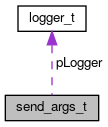
\includegraphics[width=153pt]{structsend__args__t__coll__graph}
\end{center}
\end{figure}
\subsection*{Public Attributes}
\begin{DoxyCompactItemize}
\item 
void $\ast$ \hyperlink{structsend__args__t_a1157e08ddef1b804c8609b013a14b02a}{src}
\item 
int \hyperlink{structsend__args__t_a6b05eee147bc0506bc00ab759732adba}{size}
\item 
\hyperlink{datatypes_8h_a30353f381f5fccbb956eea1f3a110b6c}{socket\+\_\+t} \hyperlink{structsend__args__t_aadc0f2cd20c6545c631d3529132c0060}{dest}
\item 
char \hyperlink{structsend__args__t_ad858929a0359a7cb06cd971619ef0baa}{name} \mbox{[}\hyperlink{datatypes_8h_ac7c0207aa5a0e10d378be03b68041350}{M\+A\+X\+\_\+\+N\+A\+ME}\mbox{]}
\item 
const \hyperlink{structlogger__t}{logger\+\_\+t} $\ast$ \hyperlink{structsend__args__t_a70fc025c17db3230f4f607415a9408e5}{p\+Logger}
\end{DoxyCompactItemize}


\subsection{Member Data Documentation}
\mbox{\Hypertarget{structsend__args__t_aadc0f2cd20c6545c631d3529132c0060}\label{structsend__args__t_aadc0f2cd20c6545c631d3529132c0060}} 
\index{send\+\_\+args\+\_\+t@{send\+\_\+args\+\_\+t}!dest@{dest}}
\index{dest@{dest}!send\+\_\+args\+\_\+t@{send\+\_\+args\+\_\+t}}
\subsubsection{\texorpdfstring{dest}{dest}}
{\footnotesize\ttfamily \hyperlink{datatypes_8h_a30353f381f5fccbb956eea1f3a110b6c}{socket\+\_\+t} send\+\_\+args\+\_\+t\+::dest}

\mbox{\Hypertarget{structsend__args__t_ad858929a0359a7cb06cd971619ef0baa}\label{structsend__args__t_ad858929a0359a7cb06cd971619ef0baa}} 
\index{send\+\_\+args\+\_\+t@{send\+\_\+args\+\_\+t}!name@{name}}
\index{name@{name}!send\+\_\+args\+\_\+t@{send\+\_\+args\+\_\+t}}
\subsubsection{\texorpdfstring{name}{name}}
{\footnotesize\ttfamily char send\+\_\+args\+\_\+t\+::name\mbox{[}\hyperlink{datatypes_8h_ac7c0207aa5a0e10d378be03b68041350}{M\+A\+X\+\_\+\+N\+A\+ME}\mbox{]}}

\mbox{\Hypertarget{structsend__args__t_a70fc025c17db3230f4f607415a9408e5}\label{structsend__args__t_a70fc025c17db3230f4f607415a9408e5}} 
\index{send\+\_\+args\+\_\+t@{send\+\_\+args\+\_\+t}!p\+Logger@{p\+Logger}}
\index{p\+Logger@{p\+Logger}!send\+\_\+args\+\_\+t@{send\+\_\+args\+\_\+t}}
\subsubsection{\texorpdfstring{p\+Logger}{pLogger}}
{\footnotesize\ttfamily const \hyperlink{structlogger__t}{logger\+\_\+t}$\ast$ send\+\_\+args\+\_\+t\+::p\+Logger}

\mbox{\Hypertarget{structsend__args__t_a6b05eee147bc0506bc00ab759732adba}\label{structsend__args__t_a6b05eee147bc0506bc00ab759732adba}} 
\index{send\+\_\+args\+\_\+t@{send\+\_\+args\+\_\+t}!size@{size}}
\index{size@{size}!send\+\_\+args\+\_\+t@{send\+\_\+args\+\_\+t}}
\subsubsection{\texorpdfstring{size}{size}}
{\footnotesize\ttfamily int send\+\_\+args\+\_\+t\+::size}

\mbox{\Hypertarget{structsend__args__t_a1157e08ddef1b804c8609b013a14b02a}\label{structsend__args__t_a1157e08ddef1b804c8609b013a14b02a}} 
\index{send\+\_\+args\+\_\+t@{send\+\_\+args\+\_\+t}!src@{src}}
\index{src@{src}!send\+\_\+args\+\_\+t@{send\+\_\+args\+\_\+t}}
\subsubsection{\texorpdfstring{src}{src}}
{\footnotesize\ttfamily void$\ast$ send\+\_\+args\+\_\+t\+::src}



The documentation for this struct was generated from the following file\+:\begin{DoxyCompactItemize}
\item 
headers/\hyperlink{protocol_8h}{protocol.\+h}\end{DoxyCompactItemize}

\hypertarget{structserver__t}{}\section{server\+\_\+t Struct Reference}
\label{structserver__t}\index{server\+\_\+t@{server\+\_\+t}}


{\ttfamily \#include $<$server.\+h$>$}

\subsection*{Data Fields}
\begin{DoxyCompactItemize}
\item 
socket\+\_\+t \hyperlink{structserver__t_a51c1726304d4644523c35656c5f9b20b}{sock}
\item 
struct sockaddr\+\_\+in \hyperlink{structserver__t_a515d831aa349c908c0a2c0e86b5e1c43}{sock\+Addr}
\item 
unsigned short \hyperlink{structserver__t_ac60a631d2267e34f3b5dd3555ae3ab43}{port}
\item 
bool \hyperlink{structserver__t_a04e5158f927016ae6577600862d8750d}{multi\+Process}
\item 
char \hyperlink{structserver__t_ae5ccab8bd0fb6744f89ae6a7e13d8553}{installation\+Dir} \mbox{[}M\+A\+X\+\_\+\+N\+A\+ME\mbox{]}
\item 
char \hyperlink{structserver__t_ac2d407054762f70d9feaf8e7998e6720}{config\+File} \mbox{[}M\+A\+X\+\_\+\+N\+A\+ME+sizeof(C\+O\+N\+F\+I\+G\+\_\+\+F\+I\+LE)\mbox{]}
\end{DoxyCompactItemize}


\subsection{Detailed Description}
A struct representing an instance of a gopher server 

\subsection{Field Documentation}
\mbox{\Hypertarget{structserver__t_ac2d407054762f70d9feaf8e7998e6720}\label{structserver__t_ac2d407054762f70d9feaf8e7998e6720}} 
\index{server\+\_\+t@{server\+\_\+t}!config\+File@{config\+File}}
\index{config\+File@{config\+File}!server\+\_\+t@{server\+\_\+t}}
\subsubsection{\texorpdfstring{config\+File}{configFile}}
{\footnotesize\ttfamily char server\+\_\+t\+::config\+File\mbox{[}M\+A\+X\+\_\+\+N\+A\+ME+sizeof(C\+O\+N\+F\+I\+G\+\_\+\+F\+I\+LE)\mbox{]}}

The server configuration file name \mbox{\Hypertarget{structserver__t_ae5ccab8bd0fb6744f89ae6a7e13d8553}\label{structserver__t_ae5ccab8bd0fb6744f89ae6a7e13d8553}} 
\index{server\+\_\+t@{server\+\_\+t}!installation\+Dir@{installation\+Dir}}
\index{installation\+Dir@{installation\+Dir}!server\+\_\+t@{server\+\_\+t}}
\subsubsection{\texorpdfstring{installation\+Dir}{installationDir}}
{\footnotesize\ttfamily char server\+\_\+t\+::installation\+Dir\mbox{[}M\+A\+X\+\_\+\+N\+A\+ME\mbox{]}}

The server main installation directory \mbox{\Hypertarget{structserver__t_a04e5158f927016ae6577600862d8750d}\label{structserver__t_a04e5158f927016ae6577600862d8750d}} 
\index{server\+\_\+t@{server\+\_\+t}!multi\+Process@{multi\+Process}}
\index{multi\+Process@{multi\+Process}!server\+\_\+t@{server\+\_\+t}}
\subsubsection{\texorpdfstring{multi\+Process}{multiProcess}}
{\footnotesize\ttfamily bool server\+\_\+t\+::multi\+Process}

A flag stating whether the server should spawn a process or a thread per request \mbox{\Hypertarget{structserver__t_ac60a631d2267e34f3b5dd3555ae3ab43}\label{structserver__t_ac60a631d2267e34f3b5dd3555ae3ab43}} 
\index{server\+\_\+t@{server\+\_\+t}!port@{port}}
\index{port@{port}!server\+\_\+t@{server\+\_\+t}}
\subsubsection{\texorpdfstring{port}{port}}
{\footnotesize\ttfamily unsigned short server\+\_\+t\+::port}

The port where the server is listening \mbox{\Hypertarget{structserver__t_a51c1726304d4644523c35656c5f9b20b}\label{structserver__t_a51c1726304d4644523c35656c5f9b20b}} 
\index{server\+\_\+t@{server\+\_\+t}!sock@{sock}}
\index{sock@{sock}!server\+\_\+t@{server\+\_\+t}}
\subsubsection{\texorpdfstring{sock}{sock}}
{\footnotesize\ttfamily socket\+\_\+t server\+\_\+t\+::sock}

The socket of the server \mbox{\Hypertarget{structserver__t_a515d831aa349c908c0a2c0e86b5e1c43}\label{structserver__t_a515d831aa349c908c0a2c0e86b5e1c43}} 
\index{server\+\_\+t@{server\+\_\+t}!sock\+Addr@{sock\+Addr}}
\index{sock\+Addr@{sock\+Addr}!server\+\_\+t@{server\+\_\+t}}
\subsubsection{\texorpdfstring{sock\+Addr}{sockAddr}}
{\footnotesize\ttfamily struct sockaddr\+\_\+in server\+\_\+t\+::sock\+Addr}

The socket address 

The documentation for this struct was generated from the following file\+:\begin{DoxyCompactItemize}
\item 
headers/\hyperlink{server_8h}{server.\+h}\end{DoxyCompactItemize}

\hypertarget{structserver__thread__args__t}{}\section{server\+\_\+thread\+\_\+args\+\_\+t Struct Reference}
\label{structserver__thread__args__t}\index{server\+\_\+thread\+\_\+args\+\_\+t@{server\+\_\+thread\+\_\+args\+\_\+t}}


{\ttfamily \#include $<$server.\+h$>$}



Collaboration diagram for server\+\_\+thread\+\_\+args\+\_\+t\+:
\nopagebreak
\begin{figure}[H]
\begin{center}
\leavevmode
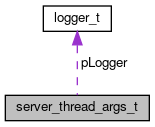
\includegraphics[width=188pt]{structserver__thread__args__t__coll__graph}
\end{center}
\end{figure}
\subsection*{Public Attributes}
\begin{DoxyCompactItemize}
\item 
\hyperlink{datatypes_8h_a30353f381f5fccbb956eea1f3a110b6c}{socket\+\_\+t} \hyperlink{structserver__thread__args__t_afcaca013fc84d1969ccb28c907ccff77}{sock}
\item 
int \hyperlink{structserver__thread__args__t_a0bf51eeb92c580aad89b8492cdb7c9bd}{port}
\item 
const \hyperlink{structlogger__t}{logger\+\_\+t} $\ast$ \hyperlink{structserver__thread__args__t_ad7c9b5025d97f79a8fbf390b9e340501}{p\+Logger}
\end{DoxyCompactItemize}


\subsection{Member Data Documentation}
\mbox{\Hypertarget{structserver__thread__args__t_ad7c9b5025d97f79a8fbf390b9e340501}\label{structserver__thread__args__t_ad7c9b5025d97f79a8fbf390b9e340501}} 
\index{server\+\_\+thread\+\_\+args\+\_\+t@{server\+\_\+thread\+\_\+args\+\_\+t}!p\+Logger@{p\+Logger}}
\index{p\+Logger@{p\+Logger}!server\+\_\+thread\+\_\+args\+\_\+t@{server\+\_\+thread\+\_\+args\+\_\+t}}
\subsubsection{\texorpdfstring{p\+Logger}{pLogger}}
{\footnotesize\ttfamily const \hyperlink{structlogger__t}{logger\+\_\+t}$\ast$ server\+\_\+thread\+\_\+args\+\_\+t\+::p\+Logger}

\mbox{\Hypertarget{structserver__thread__args__t_a0bf51eeb92c580aad89b8492cdb7c9bd}\label{structserver__thread__args__t_a0bf51eeb92c580aad89b8492cdb7c9bd}} 
\index{server\+\_\+thread\+\_\+args\+\_\+t@{server\+\_\+thread\+\_\+args\+\_\+t}!port@{port}}
\index{port@{port}!server\+\_\+thread\+\_\+args\+\_\+t@{server\+\_\+thread\+\_\+args\+\_\+t}}
\subsubsection{\texorpdfstring{port}{port}}
{\footnotesize\ttfamily int server\+\_\+thread\+\_\+args\+\_\+t\+::port}

\mbox{\Hypertarget{structserver__thread__args__t_afcaca013fc84d1969ccb28c907ccff77}\label{structserver__thread__args__t_afcaca013fc84d1969ccb28c907ccff77}} 
\index{server\+\_\+thread\+\_\+args\+\_\+t@{server\+\_\+thread\+\_\+args\+\_\+t}!sock@{sock}}
\index{sock@{sock}!server\+\_\+thread\+\_\+args\+\_\+t@{server\+\_\+thread\+\_\+args\+\_\+t}}
\subsubsection{\texorpdfstring{sock}{sock}}
{\footnotesize\ttfamily \hyperlink{datatypes_8h_a30353f381f5fccbb956eea1f3a110b6c}{socket\+\_\+t} server\+\_\+thread\+\_\+args\+\_\+t\+::sock}



The documentation for this struct was generated from the following file\+:\begin{DoxyCompactItemize}
\item 
headers/\hyperlink{server_8h}{server.\+h}\end{DoxyCompactItemize}

\chapter{File Documentation}
\hypertarget{constants_8h}{}\section{headers/constants.h File Reference}
\label{constants_8h}\index{headers/constants.\+h@{headers/constants.\+h}}
\subsection*{Macros}
\begin{DoxyCompactItemize}
\item 
\#define \hyperlink{constants_8h_a26769957ec1a2beaf223f33b66ee64ab}{I\+N\+V\+A\+L\+I\+D\+\_\+\+S\+O\+C\+K\+ET}~-\/1
\item 
\#define \hyperlink{constants_8h_a633b0396ff93d336a088412a190a5072}{S\+O\+C\+K\+E\+T\+\_\+\+E\+R\+R\+OR}~-\/1
\item 
\#define \hyperlink{constants_8h_aa7b44c9aa2f59f8e56950979bfafe4c6}{I\+P\+\_\+\+A\+D\+D\+R\+E\+S\+S\+\_\+\+L\+E\+N\+G\+TH}~16
\end{DoxyCompactItemize}


\subsection{Macro Definition Documentation}
\mbox{\Hypertarget{constants_8h_a26769957ec1a2beaf223f33b66ee64ab}\label{constants_8h_a26769957ec1a2beaf223f33b66ee64ab}} 
\index{constants.\+h@{constants.\+h}!I\+N\+V\+A\+L\+I\+D\+\_\+\+S\+O\+C\+K\+ET@{I\+N\+V\+A\+L\+I\+D\+\_\+\+S\+O\+C\+K\+ET}}
\index{I\+N\+V\+A\+L\+I\+D\+\_\+\+S\+O\+C\+K\+ET@{I\+N\+V\+A\+L\+I\+D\+\_\+\+S\+O\+C\+K\+ET}!constants.\+h@{constants.\+h}}
\subsubsection{\texorpdfstring{I\+N\+V\+A\+L\+I\+D\+\_\+\+S\+O\+C\+K\+ET}{INVALID\_SOCKET}}
{\footnotesize\ttfamily \#define I\+N\+V\+A\+L\+I\+D\+\_\+\+S\+O\+C\+K\+ET~-\/1}

\mbox{\Hypertarget{constants_8h_aa7b44c9aa2f59f8e56950979bfafe4c6}\label{constants_8h_aa7b44c9aa2f59f8e56950979bfafe4c6}} 
\index{constants.\+h@{constants.\+h}!I\+P\+\_\+\+A\+D\+D\+R\+E\+S\+S\+\_\+\+L\+E\+N\+G\+TH@{I\+P\+\_\+\+A\+D\+D\+R\+E\+S\+S\+\_\+\+L\+E\+N\+G\+TH}}
\index{I\+P\+\_\+\+A\+D\+D\+R\+E\+S\+S\+\_\+\+L\+E\+N\+G\+TH@{I\+P\+\_\+\+A\+D\+D\+R\+E\+S\+S\+\_\+\+L\+E\+N\+G\+TH}!constants.\+h@{constants.\+h}}
\subsubsection{\texorpdfstring{I\+P\+\_\+\+A\+D\+D\+R\+E\+S\+S\+\_\+\+L\+E\+N\+G\+TH}{IP\_ADDRESS\_LENGTH}}
{\footnotesize\ttfamily \#define I\+P\+\_\+\+A\+D\+D\+R\+E\+S\+S\+\_\+\+L\+E\+N\+G\+TH~16}

\mbox{\Hypertarget{constants_8h_a633b0396ff93d336a088412a190a5072}\label{constants_8h_a633b0396ff93d336a088412a190a5072}} 
\index{constants.\+h@{constants.\+h}!S\+O\+C\+K\+E\+T\+\_\+\+E\+R\+R\+OR@{S\+O\+C\+K\+E\+T\+\_\+\+E\+R\+R\+OR}}
\index{S\+O\+C\+K\+E\+T\+\_\+\+E\+R\+R\+OR@{S\+O\+C\+K\+E\+T\+\_\+\+E\+R\+R\+OR}!constants.\+h@{constants.\+h}}
\subsubsection{\texorpdfstring{S\+O\+C\+K\+E\+T\+\_\+\+E\+R\+R\+OR}{SOCKET\_ERROR}}
{\footnotesize\ttfamily \#define S\+O\+C\+K\+E\+T\+\_\+\+E\+R\+R\+OR~-\/1}


\hypertarget{datatypes_8h}{}\section{headers/datatypes.h File Reference}
\label{datatypes_8h}\index{headers/datatypes.\+h@{headers/datatypes.\+h}}
{\ttfamily \#include $<$dirent.\+h$>$}\newline
{\ttfamily \#include $<$signal.\+h$>$}\newline
{\ttfamily \#include $<$stdbool.\+h$>$}\newline
{\ttfamily \#include $<$stdio.\+h$>$}\newline
{\ttfamily \#include $<$sys/stat.\+h$>$}\newline
{\ttfamily \#include $<$sys/types.\+h$>$}\newline
Include dependency graph for datatypes.\+h\+:\nopagebreak
\begin{figure}[H]
\begin{center}
\leavevmode
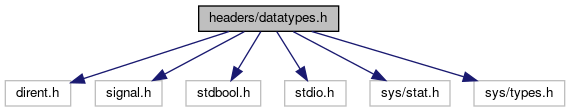
\includegraphics[width=350pt]{datatypes_8h__incl}
\end{center}
\end{figure}
This graph shows which files directly or indirectly include this file\+:\nopagebreak
\begin{figure}[H]
\begin{center}
\leavevmode
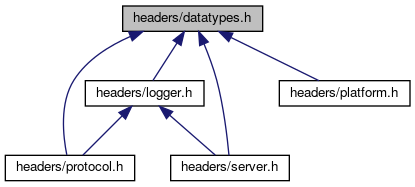
\includegraphics[width=350pt]{datatypes_8h__dep__incl}
\end{center}
\end{figure}
\subsection*{Macros}
\begin{DoxyCompactItemize}
\item 
\#define \hyperlink{datatypes_8h_ac7c0207aa5a0e10d378be03b68041350}{M\+A\+X\+\_\+\+N\+A\+ME}~F\+I\+L\+E\+N\+A\+M\+E\+\_\+\+M\+AX
\end{DoxyCompactItemize}
\subsection*{Typedefs}
\begin{DoxyCompactItemize}
\item 
typedef int \hyperlink{datatypes_8h_a30353f381f5fccbb956eea1f3a110b6c}{socket\+\_\+t}
\item 
typedef int \hyperlink{datatypes_8h_aaf06dbc1f07c15cb5e2779d3ec2dcb4b}{event\+\_\+t}
\item 
typedef int \hyperlink{datatypes_8h_ad37b29694b7e5ee41ea19673078dc995}{pipe\+\_\+t}
\item 
typedef char $\ast$ \hyperlink{datatypes_8h_ab0dcbec9b4b3c60b939b1095f93cb1b9}{string\+\_\+t}
\item 
typedef const char $\ast$ \hyperlink{datatypes_8h_a64c80a7679fadd808852566a2af0dd52}{cstring\+\_\+t}
\item 
typedef void \hyperlink{datatypes_8h_aad926342f971218b81db6fed8012f78f}{\+\_\+handler\+Ret}
\item 
typedef pthread\+\_\+t \hyperlink{datatypes_8h_aa406fd87cfd69d7c0a93b6a241978712}{thread\+\_\+t}
\item 
typedef void $\ast$($\ast$ \hyperlink{datatypes_8h_a0b51ef0c937612d03100482d10a01222}{L\+P\+T\+H\+R\+E\+A\+D\+\_\+\+S\+T\+A\+R\+T\+\_\+\+R\+O\+U\+T\+I\+NE}) (void $\ast$)
\item 
typedef sig\+\_\+atomic\+\_\+t \hyperlink{datatypes_8h_a23ea32a60b3b734eae2c0a9e75d3397c}{sig\+\_\+atomic}
\item 
typedef D\+IR $\ast$ \hyperlink{datatypes_8h_ae4a73300ce565f1cf992f892f5c2d0c0}{\+\_\+dir}
\item 
typedef pthread\+\_\+mutex\+\_\+t \hyperlink{datatypes_8h_a6bfdd7a014fe4d4d6c392df201d822dd}{mutex\+\_\+t}
\item 
typedef pthread\+\_\+cond\+\_\+t \hyperlink{datatypes_8h_ab9991f7052428330da4c2fb771e0439f}{cond\+\_\+t}
\item 
typedef pid\+\_\+t \hyperlink{datatypes_8h_a03c58ad8bfbf8e14928e8f58a5f23f2e}{proc\+\_\+id\+\_\+t}
\end{DoxyCompactItemize}


\subsection{Macro Definition Documentation}
\mbox{\Hypertarget{datatypes_8h_ac7c0207aa5a0e10d378be03b68041350}\label{datatypes_8h_ac7c0207aa5a0e10d378be03b68041350}} 
\index{datatypes.\+h@{datatypes.\+h}!M\+A\+X\+\_\+\+N\+A\+ME@{M\+A\+X\+\_\+\+N\+A\+ME}}
\index{M\+A\+X\+\_\+\+N\+A\+ME@{M\+A\+X\+\_\+\+N\+A\+ME}!datatypes.\+h@{datatypes.\+h}}
\subsubsection{\texorpdfstring{M\+A\+X\+\_\+\+N\+A\+ME}{MAX\_NAME}}
{\footnotesize\ttfamily \#define M\+A\+X\+\_\+\+N\+A\+ME~F\+I\+L\+E\+N\+A\+M\+E\+\_\+\+M\+AX}



\subsection{Typedef Documentation}
\mbox{\Hypertarget{datatypes_8h_ae4a73300ce565f1cf992f892f5c2d0c0}\label{datatypes_8h_ae4a73300ce565f1cf992f892f5c2d0c0}} 
\index{datatypes.\+h@{datatypes.\+h}!\+\_\+dir@{\+\_\+dir}}
\index{\+\_\+dir@{\+\_\+dir}!datatypes.\+h@{datatypes.\+h}}
\subsubsection{\texorpdfstring{\+\_\+dir}{\_dir}}
{\footnotesize\ttfamily typedef D\+IR$\ast$ \hyperlink{datatypes_8h_ae4a73300ce565f1cf992f892f5c2d0c0}{\+\_\+dir}}

\mbox{\Hypertarget{datatypes_8h_aad926342f971218b81db6fed8012f78f}\label{datatypes_8h_aad926342f971218b81db6fed8012f78f}} 
\index{datatypes.\+h@{datatypes.\+h}!\+\_\+handler\+Ret@{\+\_\+handler\+Ret}}
\index{\+\_\+handler\+Ret@{\+\_\+handler\+Ret}!datatypes.\+h@{datatypes.\+h}}
\subsubsection{\texorpdfstring{\+\_\+handler\+Ret}{\_handlerRet}}
{\footnotesize\ttfamily typedef void \hyperlink{datatypes_8h_aad926342f971218b81db6fed8012f78f}{\+\_\+handler\+Ret}}

\mbox{\Hypertarget{datatypes_8h_ab9991f7052428330da4c2fb771e0439f}\label{datatypes_8h_ab9991f7052428330da4c2fb771e0439f}} 
\index{datatypes.\+h@{datatypes.\+h}!cond\+\_\+t@{cond\+\_\+t}}
\index{cond\+\_\+t@{cond\+\_\+t}!datatypes.\+h@{datatypes.\+h}}
\subsubsection{\texorpdfstring{cond\+\_\+t}{cond\_t}}
{\footnotesize\ttfamily typedef pthread\+\_\+cond\+\_\+t \hyperlink{datatypes_8h_ab9991f7052428330da4c2fb771e0439f}{cond\+\_\+t}}

\mbox{\Hypertarget{datatypes_8h_a64c80a7679fadd808852566a2af0dd52}\label{datatypes_8h_a64c80a7679fadd808852566a2af0dd52}} 
\index{datatypes.\+h@{datatypes.\+h}!cstring\+\_\+t@{cstring\+\_\+t}}
\index{cstring\+\_\+t@{cstring\+\_\+t}!datatypes.\+h@{datatypes.\+h}}
\subsubsection{\texorpdfstring{cstring\+\_\+t}{cstring\_t}}
{\footnotesize\ttfamily typedef const char$\ast$ \hyperlink{datatypes_8h_a64c80a7679fadd808852566a2af0dd52}{cstring\+\_\+t}}

\mbox{\Hypertarget{datatypes_8h_aaf06dbc1f07c15cb5e2779d3ec2dcb4b}\label{datatypes_8h_aaf06dbc1f07c15cb5e2779d3ec2dcb4b}} 
\index{datatypes.\+h@{datatypes.\+h}!event\+\_\+t@{event\+\_\+t}}
\index{event\+\_\+t@{event\+\_\+t}!datatypes.\+h@{datatypes.\+h}}
\subsubsection{\texorpdfstring{event\+\_\+t}{event\_t}}
{\footnotesize\ttfamily typedef int \hyperlink{datatypes_8h_aaf06dbc1f07c15cb5e2779d3ec2dcb4b}{event\+\_\+t}}

\mbox{\Hypertarget{datatypes_8h_a0b51ef0c937612d03100482d10a01222}\label{datatypes_8h_a0b51ef0c937612d03100482d10a01222}} 
\index{datatypes.\+h@{datatypes.\+h}!L\+P\+T\+H\+R\+E\+A\+D\+\_\+\+S\+T\+A\+R\+T\+\_\+\+R\+O\+U\+T\+I\+NE@{L\+P\+T\+H\+R\+E\+A\+D\+\_\+\+S\+T\+A\+R\+T\+\_\+\+R\+O\+U\+T\+I\+NE}}
\index{L\+P\+T\+H\+R\+E\+A\+D\+\_\+\+S\+T\+A\+R\+T\+\_\+\+R\+O\+U\+T\+I\+NE@{L\+P\+T\+H\+R\+E\+A\+D\+\_\+\+S\+T\+A\+R\+T\+\_\+\+R\+O\+U\+T\+I\+NE}!datatypes.\+h@{datatypes.\+h}}
\subsubsection{\texorpdfstring{L\+P\+T\+H\+R\+E\+A\+D\+\_\+\+S\+T\+A\+R\+T\+\_\+\+R\+O\+U\+T\+I\+NE}{LPTHREAD\_START\_ROUTINE}}
{\footnotesize\ttfamily typedef void$\ast$($\ast$ L\+P\+T\+H\+R\+E\+A\+D\+\_\+\+S\+T\+A\+R\+T\+\_\+\+R\+O\+U\+T\+I\+NE) (void $\ast$)}

\mbox{\Hypertarget{datatypes_8h_a6bfdd7a014fe4d4d6c392df201d822dd}\label{datatypes_8h_a6bfdd7a014fe4d4d6c392df201d822dd}} 
\index{datatypes.\+h@{datatypes.\+h}!mutex\+\_\+t@{mutex\+\_\+t}}
\index{mutex\+\_\+t@{mutex\+\_\+t}!datatypes.\+h@{datatypes.\+h}}
\subsubsection{\texorpdfstring{mutex\+\_\+t}{mutex\_t}}
{\footnotesize\ttfamily typedef pthread\+\_\+mutex\+\_\+t \hyperlink{datatypes_8h_a6bfdd7a014fe4d4d6c392df201d822dd}{mutex\+\_\+t}}

\mbox{\Hypertarget{datatypes_8h_ad37b29694b7e5ee41ea19673078dc995}\label{datatypes_8h_ad37b29694b7e5ee41ea19673078dc995}} 
\index{datatypes.\+h@{datatypes.\+h}!pipe\+\_\+t@{pipe\+\_\+t}}
\index{pipe\+\_\+t@{pipe\+\_\+t}!datatypes.\+h@{datatypes.\+h}}
\subsubsection{\texorpdfstring{pipe\+\_\+t}{pipe\_t}}
{\footnotesize\ttfamily typedef int \hyperlink{datatypes_8h_ad37b29694b7e5ee41ea19673078dc995}{pipe\+\_\+t}}

\mbox{\Hypertarget{datatypes_8h_a03c58ad8bfbf8e14928e8f58a5f23f2e}\label{datatypes_8h_a03c58ad8bfbf8e14928e8f58a5f23f2e}} 
\index{datatypes.\+h@{datatypes.\+h}!proc\+\_\+id\+\_\+t@{proc\+\_\+id\+\_\+t}}
\index{proc\+\_\+id\+\_\+t@{proc\+\_\+id\+\_\+t}!datatypes.\+h@{datatypes.\+h}}
\subsubsection{\texorpdfstring{proc\+\_\+id\+\_\+t}{proc\_id\_t}}
{\footnotesize\ttfamily typedef pid\+\_\+t \hyperlink{datatypes_8h_a03c58ad8bfbf8e14928e8f58a5f23f2e}{proc\+\_\+id\+\_\+t}}

\mbox{\Hypertarget{datatypes_8h_a23ea32a60b3b734eae2c0a9e75d3397c}\label{datatypes_8h_a23ea32a60b3b734eae2c0a9e75d3397c}} 
\index{datatypes.\+h@{datatypes.\+h}!sig\+\_\+atomic@{sig\+\_\+atomic}}
\index{sig\+\_\+atomic@{sig\+\_\+atomic}!datatypes.\+h@{datatypes.\+h}}
\subsubsection{\texorpdfstring{sig\+\_\+atomic}{sig\_atomic}}
{\footnotesize\ttfamily typedef sig\+\_\+atomic\+\_\+t \hyperlink{datatypes_8h_a23ea32a60b3b734eae2c0a9e75d3397c}{sig\+\_\+atomic}}

\mbox{\Hypertarget{datatypes_8h_a30353f381f5fccbb956eea1f3a110b6c}\label{datatypes_8h_a30353f381f5fccbb956eea1f3a110b6c}} 
\index{datatypes.\+h@{datatypes.\+h}!socket\+\_\+t@{socket\+\_\+t}}
\index{socket\+\_\+t@{socket\+\_\+t}!datatypes.\+h@{datatypes.\+h}}
\subsubsection{\texorpdfstring{socket\+\_\+t}{socket\_t}}
{\footnotesize\ttfamily typedef int \hyperlink{datatypes_8h_a30353f381f5fccbb956eea1f3a110b6c}{socket\+\_\+t}}

\mbox{\Hypertarget{datatypes_8h_ab0dcbec9b4b3c60b939b1095f93cb1b9}\label{datatypes_8h_ab0dcbec9b4b3c60b939b1095f93cb1b9}} 
\index{datatypes.\+h@{datatypes.\+h}!string\+\_\+t@{string\+\_\+t}}
\index{string\+\_\+t@{string\+\_\+t}!datatypes.\+h@{datatypes.\+h}}
\subsubsection{\texorpdfstring{string\+\_\+t}{string\_t}}
{\footnotesize\ttfamily typedef char$\ast$ \hyperlink{datatypes_8h_ab0dcbec9b4b3c60b939b1095f93cb1b9}{string\+\_\+t}}

\mbox{\Hypertarget{datatypes_8h_aa406fd87cfd69d7c0a93b6a241978712}\label{datatypes_8h_aa406fd87cfd69d7c0a93b6a241978712}} 
\index{datatypes.\+h@{datatypes.\+h}!thread\+\_\+t@{thread\+\_\+t}}
\index{thread\+\_\+t@{thread\+\_\+t}!datatypes.\+h@{datatypes.\+h}}
\subsubsection{\texorpdfstring{thread\+\_\+t}{thread\_t}}
{\footnotesize\ttfamily typedef pthread\+\_\+t \hyperlink{datatypes_8h_aa406fd87cfd69d7c0a93b6a241978712}{thread\+\_\+t}}


\hypertarget{log_8h}{}\section{headers/log.h File Reference}
\label{log_8h}\index{headers/log.\+h@{headers/log.\+h}}
This graph shows which files directly or indirectly include this file\+:\nopagebreak
\begin{figure}[H]
\begin{center}
\leavevmode
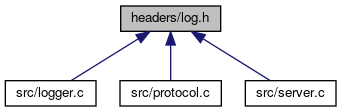
\includegraphics[width=328pt]{log_8h__dep__incl}
\end{center}
\end{figure}


\subsection{Detailed Description}
Contains constant messages for logging. 
\hypertarget{logger_8h}{}\section{headers/logger.h File Reference}
\label{logger_8h}\index{headers/logger.\+h@{headers/logger.\+h}}
{\ttfamily \#include \char`\"{}datatypes.\+h\char`\"{}}\newline
Include dependency graph for logger.\+h\+:\nopagebreak
\begin{figure}[H]
\begin{center}
\leavevmode
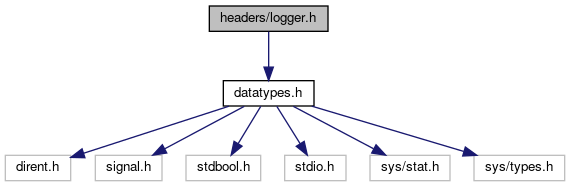
\includegraphics[width=350pt]{logger_8h__incl}
\end{center}
\end{figure}
This graph shows which files directly or indirectly include this file\+:\nopagebreak
\begin{figure}[H]
\begin{center}
\leavevmode
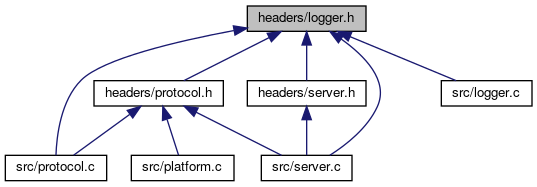
\includegraphics[width=350pt]{logger_8h__dep__incl}
\end{center}
\end{figure}
\subsection*{Data Structures}
\begin{DoxyCompactItemize}
\item 
struct \hyperlink{structlogger__t}{logger\+\_\+t}
\end{DoxyCompactItemize}
\subsection*{Functions}
\begin{DoxyCompactItemize}
\item 
int \hyperlink{logger_8h_a568bb98500e52ddc98667703cdc46927}{start\+Transfer\+Log} (\hyperlink{structlogger__t}{logger\+\_\+t} $\ast$p\+Logger)
\item 
int \hyperlink{logger_8h_a5a3ad1e6309f96bc43ab8e56ea8ffd39}{stop\+Transfer\+Log} (\hyperlink{structlogger__t}{logger\+\_\+t} $\ast$p\+Logger)
\item 
int \hyperlink{logger_8h_a75e89b9eefc53e23a458412ea544ab7e}{log\+Transfer} (const \hyperlink{structlogger__t}{logger\+\_\+t} $\ast$p\+Logger, cstring\+\_\+t log)
\end{DoxyCompactItemize}


\subsection{Detailed Description}
Functions to handle the logging of the gopher file transfers. 

\subsection{Function Documentation}
\mbox{\Hypertarget{logger_8h_a75e89b9eefc53e23a458412ea544ab7e}\label{logger_8h_a75e89b9eefc53e23a458412ea544ab7e}} 
\index{logger.\+h@{logger.\+h}!log\+Transfer@{log\+Transfer}}
\index{log\+Transfer@{log\+Transfer}!logger.\+h@{logger.\+h}}
\subsubsection{\texorpdfstring{log\+Transfer()}{logTransfer()}}
{\footnotesize\ttfamily int log\+Transfer (\begin{DoxyParamCaption}\item[{const \hyperlink{structlogger__t}{logger\+\_\+t} $\ast$}]{p\+Logger,  }\item[{cstring\+\_\+t}]{log }\end{DoxyParamCaption})}

Passes a message to a logging process. 
\begin{DoxyParams}{Parameters}
{\em p\+Logger} & The struct representing the logging process. \\
\hline
{\em log} & The message to log. \\
\hline
\end{DoxyParams}
\begin{DoxyReturn}{Returns}
L\+O\+G\+G\+E\+R\+\_\+\+S\+U\+C\+C\+E\+SS or L\+O\+G\+G\+E\+R\+\_\+\+F\+A\+I\+L\+U\+RE. 
\end{DoxyReturn}
\begin{DoxySeeAlso}{See also}
\hyperlink{structlogger__t}{logger\+\_\+t} 
\end{DoxySeeAlso}
\mbox{\Hypertarget{logger_8h_a568bb98500e52ddc98667703cdc46927}\label{logger_8h_a568bb98500e52ddc98667703cdc46927}} 
\index{logger.\+h@{logger.\+h}!start\+Transfer\+Log@{start\+Transfer\+Log}}
\index{start\+Transfer\+Log@{start\+Transfer\+Log}!logger.\+h@{logger.\+h}}
\subsubsection{\texorpdfstring{start\+Transfer\+Log()}{startTransferLog()}}
{\footnotesize\ttfamily int start\+Transfer\+Log (\begin{DoxyParamCaption}\item[{\hyperlink{structlogger__t}{logger\+\_\+t} $\ast$}]{p\+Logger }\end{DoxyParamCaption})}

Starts a logging process and writes its information in a \hyperlink{structlogger__t}{logger\+\_\+t} struct. 
\begin{DoxyParams}{Parameters}
{\em p\+Logger} & The struct that will contain information about the logger. \\
\hline
\end{DoxyParams}
\begin{DoxyReturn}{Returns}
L\+O\+G\+G\+E\+R\+\_\+\+S\+U\+C\+C\+E\+SS or L\+O\+G\+G\+E\+R\+\_\+\+F\+A\+I\+L\+U\+RE. 
\end{DoxyReturn}
\begin{DoxySeeAlso}{See also}
\hyperlink{structlogger__t}{logger\+\_\+t} 
\end{DoxySeeAlso}
\mbox{\Hypertarget{logger_8h_a5a3ad1e6309f96bc43ab8e56ea8ffd39}\label{logger_8h_a5a3ad1e6309f96bc43ab8e56ea8ffd39}} 
\index{logger.\+h@{logger.\+h}!stop\+Transfer\+Log@{stop\+Transfer\+Log}}
\index{stop\+Transfer\+Log@{stop\+Transfer\+Log}!logger.\+h@{logger.\+h}}
\subsubsection{\texorpdfstring{stop\+Transfer\+Log()}{stopTransferLog()}}
{\footnotesize\ttfamily int stop\+Transfer\+Log (\begin{DoxyParamCaption}\item[{\hyperlink{structlogger__t}{logger\+\_\+t} $\ast$}]{p\+Logger }\end{DoxyParamCaption})}

Stops a logging process. N\+O\+TE\+: Be sure to initialize the \hyperlink{structlogger__t}{logger\+\_\+t} struct by calling \hyperlink{logger_8h_a568bb98500e52ddc98667703cdc46927}{start\+Transfer\+Log()}. 
\begin{DoxyParams}{Parameters}
{\em p\+Logger} & A pointer to the struct representing the logger process to stop. \\
\hline
\end{DoxyParams}
\begin{DoxyReturn}{Returns}
L\+O\+G\+G\+E\+R\+\_\+\+S\+U\+C\+C\+E\+SS or L\+O\+G\+G\+E\+R\+\_\+\+F\+A\+I\+L\+U\+RE. 
\end{DoxyReturn}
\begin{DoxySeeAlso}{See also}
\hyperlink{structlogger__t}{logger\+\_\+t} 
\end{DoxySeeAlso}

\hypertarget{platform_8h}{}\section{headers/platform.h File Reference}
\label{platform_8h}\index{headers/platform.\+h@{headers/platform.\+h}}
{\ttfamily \#include $<$arpa/inet.\+h$>$}\newline
{\ttfamily \#include $<$netinet/in.\+h$>$}\newline
{\ttfamily \#include $<$syslog.\+h$>$}\newline
{\ttfamily \#include $<$stdbool.\+h$>$}\newline
{\ttfamily \#include $<$stdlib.\+h$>$}\newline
{\ttfamily \#include \char`\"{}datatypes.\+h\char`\"{}}\newline
Include dependency graph for platform.\+h\+:\nopagebreak
\begin{figure}[H]
\begin{center}
\leavevmode
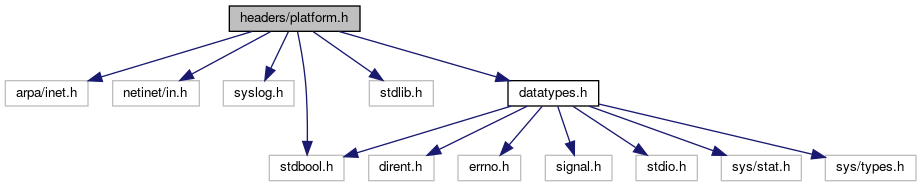
\includegraphics[width=350pt]{platform_8h__incl}
\end{center}
\end{figure}
\subsection*{Classes}
\begin{DoxyCompactItemize}
\item 
struct \hyperlink{structfile__mapping__t}{file\+\_\+mapping\+\_\+t}
\end{DoxyCompactItemize}
\subsection*{Macros}
\begin{DoxyCompactItemize}
\item 
\#define \hyperlink{platform_8h_a26769957ec1a2beaf223f33b66ee64ab}{I\+N\+V\+A\+L\+I\+D\+\_\+\+S\+O\+C\+K\+ET}~-\/1
\item 
\#define \hyperlink{platform_8h_a633b0396ff93d336a088412a190a5072}{S\+O\+C\+K\+E\+T\+\_\+\+E\+R\+R\+OR}~-\/1
\item 
\#define \hyperlink{platform_8h_a8283f9200dc6b46f340efb3915720220}{P\+L\+A\+T\+F\+O\+R\+M\+\_\+\+S\+U\+C\+C\+E\+SS}~0x0000
\item 
\#define \hyperlink{platform_8h_a37daedd859593e5563c9fb133b899091}{P\+L\+A\+T\+F\+O\+R\+M\+\_\+\+F\+A\+I\+L\+U\+RE}~0x0001
\item 
\#define \hyperlink{platform_8h_ac6e7400254a5d386ad20bff6add48c9e}{P\+L\+A\+T\+F\+O\+R\+M\+\_\+\+F\+I\+L\+E\+\_\+\+E\+RR}~0x0001
\item 
\#define \hyperlink{platform_8h_a316e63ab4300a66d11278243296732d9}{P\+L\+A\+T\+F\+O\+R\+M\+\_\+\+I\+S\+F\+I\+LE}~0x0002
\item 
\#define \hyperlink{platform_8h_ab7d909f67b15866719974afa696d0185}{P\+L\+A\+T\+F\+O\+R\+M\+\_\+\+I\+S\+D\+IR}~0x0004
\item 
\#define \hyperlink{platform_8h_a40502f8021fe7e3c327d7a61a54a8608}{P\+L\+A\+T\+F\+O\+R\+M\+\_\+\+N\+O\+T\+\_\+\+F\+O\+U\+ND}~0x0008
\item 
\#define \hyperlink{platform_8h_a0ea5ffbd94c6f72156a767ad0ab80728}{P\+L\+A\+T\+F\+O\+R\+M\+\_\+\+E\+N\+D\+\_\+\+O\+F\+\_\+\+D\+IR}~0x0010
\end{DoxyCompactItemize}
\subsection*{Functions}
\begin{DoxyCompactItemize}
\item 
bool \hyperlink{platform_8h_a2b652b5d50088ca766e09ba7115e9a9e}{ends\+With} (\hyperlink{datatypes_8h_a64c80a7679fadd808852566a2af0dd52}{cstring\+\_\+t} str1, \hyperlink{datatypes_8h_a64c80a7679fadd808852566a2af0dd52}{cstring\+\_\+t} str2)
\item 
int \hyperlink{platform_8h_ab296265b5db20ab2f30dd1e985dc64aa}{get\+Cwd} (\hyperlink{datatypes_8h_ab0dcbec9b4b3c60b939b1095f93cb1b9}{string\+\_\+t} dst, size\+\_\+t size)
\item 
int \hyperlink{platform_8h_aaba941b4423e015bc9dd4a9cad5a8363}{change\+Cwd} (\hyperlink{datatypes_8h_a64c80a7679fadd808852566a2af0dd52}{cstring\+\_\+t} path)
\item 
void \hyperlink{platform_8h_a4e984a09b582ada83d582322f65c9d1a}{log\+Message} (\hyperlink{datatypes_8h_a64c80a7679fadd808852566a2af0dd52}{cstring\+\_\+t} message, int level)
\item 
int \hyperlink{platform_8h_a365b2a06835658e622a46fa55036cdc3}{sock\+Err} ()
\item 
int \hyperlink{platform_8h_a9056a7cd4a35131aa7e8094fc897774c}{close\+Socket} (\hyperlink{datatypes_8h_a30353f381f5fccbb956eea1f3a110b6c}{socket\+\_\+t} s)
\item 
int \hyperlink{platform_8h_adb504f94873e3ed50a9fbc948b3f6244}{send\+All} (\hyperlink{datatypes_8h_a30353f381f5fccbb956eea1f3a110b6c}{socket\+\_\+t} s, \hyperlink{datatypes_8h_a64c80a7679fadd808852566a2af0dd52}{cstring\+\_\+t} data, int length)
\item 
\hyperlink{datatypes_8h_a64c80a7679fadd808852566a2af0dd52}{cstring\+\_\+t} \hyperlink{platform_8h_ab01622372f7ef0249efabdfdc26d240b}{inet\+Ntoa} (const struct in\+\_\+addr $\ast$addr, void $\ast$dst, size\+\_\+t size)
\item 
int \hyperlink{platform_8h_a5ff45f4458f458d37d427bf5e676f22a}{file\+Attributes} (\hyperlink{datatypes_8h_a64c80a7679fadd808852566a2af0dd52}{cstring\+\_\+t} path)
\item 
int \hyperlink{platform_8h_afc7e96be2f7333bcc10813fdebcf124a}{get\+File\+Size} (\hyperlink{datatypes_8h_a64c80a7679fadd808852566a2af0dd52}{cstring\+\_\+t} path)
\item 
int \hyperlink{platform_8h_a0cec7649e32d72daadab4beb95e6ef96}{iterate\+Dir} (\hyperlink{datatypes_8h_a64c80a7679fadd808852566a2af0dd52}{cstring\+\_\+t} path, \hyperlink{datatypes_8h_ae4a73300ce565f1cf992f892f5c2d0c0}{\+\_\+dir} $\ast$dir, \hyperlink{datatypes_8h_ab0dcbec9b4b3c60b939b1095f93cb1b9}{string\+\_\+t} name, size\+\_\+t name\+Size)
\item 
int \hyperlink{platform_8h_a89df221b2d4303be5ae36c1ab470716d}{close\+Dir} (\hyperlink{datatypes_8h_ae4a73300ce565f1cf992f892f5c2d0c0}{\+\_\+dir} dir)
\item 
int \hyperlink{platform_8h_a257d48e91fab744f0f71ad79f5acfef2}{get\+File\+Map} (\hyperlink{datatypes_8h_a64c80a7679fadd808852566a2af0dd52}{cstring\+\_\+t} path, \hyperlink{structfile__mapping__t}{file\+\_\+mapping\+\_\+t} $\ast$map\+Data)
\item 
int \hyperlink{platform_8h_a3a359d5a433a1e941b0f312bf1cd15ef}{unmap\+Mem} (void $\ast$addr, size\+\_\+t len)
\item 
int \hyperlink{platform_8h_a6c4fe83342c470fa5b3b79277f65bfa3}{start\+Thread} (\hyperlink{datatypes_8h_aa406fd87cfd69d7c0a93b6a241978712}{thread\+\_\+t} $\ast$tid, \hyperlink{datatypes_8h_a0b51ef0c937612d03100482d10a01222}{L\+P\+T\+H\+R\+E\+A\+D\+\_\+\+S\+T\+A\+R\+T\+\_\+\+R\+O\+U\+T\+I\+NE} routine, void $\ast$args)
\item 
int \hyperlink{platform_8h_a4488400062d2d5378e371cacc7b5b94c}{detach\+Thread} (\hyperlink{datatypes_8h_aa406fd87cfd69d7c0a93b6a241978712}{thread\+\_\+t} tid)
\item 
int \hyperlink{platform_8h_afd3d7cf7c06200399620828a2e44a0e1}{daemonize} ()
\item 
void \hyperlink{platform_8h_a56c0ddfef7f02bfb28f31d5011380730}{debug\+Pause} (\hyperlink{datatypes_8h_a64c80a7679fadd808852566a2af0dd52}{cstring\+\_\+t} message)
\end{DoxyCompactItemize}


\subsection{Macro Definition Documentation}
\mbox{\Hypertarget{platform_8h_a26769957ec1a2beaf223f33b66ee64ab}\label{platform_8h_a26769957ec1a2beaf223f33b66ee64ab}} 
\index{platform.\+h@{platform.\+h}!I\+N\+V\+A\+L\+I\+D\+\_\+\+S\+O\+C\+K\+ET@{I\+N\+V\+A\+L\+I\+D\+\_\+\+S\+O\+C\+K\+ET}}
\index{I\+N\+V\+A\+L\+I\+D\+\_\+\+S\+O\+C\+K\+ET@{I\+N\+V\+A\+L\+I\+D\+\_\+\+S\+O\+C\+K\+ET}!platform.\+h@{platform.\+h}}
\subsubsection{\texorpdfstring{I\+N\+V\+A\+L\+I\+D\+\_\+\+S\+O\+C\+K\+ET}{INVALID\_SOCKET}}
{\footnotesize\ttfamily \#define I\+N\+V\+A\+L\+I\+D\+\_\+\+S\+O\+C\+K\+ET~-\/1}

\mbox{\Hypertarget{platform_8h_a0ea5ffbd94c6f72156a767ad0ab80728}\label{platform_8h_a0ea5ffbd94c6f72156a767ad0ab80728}} 
\index{platform.\+h@{platform.\+h}!P\+L\+A\+T\+F\+O\+R\+M\+\_\+\+E\+N\+D\+\_\+\+O\+F\+\_\+\+D\+IR@{P\+L\+A\+T\+F\+O\+R\+M\+\_\+\+E\+N\+D\+\_\+\+O\+F\+\_\+\+D\+IR}}
\index{P\+L\+A\+T\+F\+O\+R\+M\+\_\+\+E\+N\+D\+\_\+\+O\+F\+\_\+\+D\+IR@{P\+L\+A\+T\+F\+O\+R\+M\+\_\+\+E\+N\+D\+\_\+\+O\+F\+\_\+\+D\+IR}!platform.\+h@{platform.\+h}}
\subsubsection{\texorpdfstring{P\+L\+A\+T\+F\+O\+R\+M\+\_\+\+E\+N\+D\+\_\+\+O\+F\+\_\+\+D\+IR}{PLATFORM\_END\_OF\_DIR}}
{\footnotesize\ttfamily \#define P\+L\+A\+T\+F\+O\+R\+M\+\_\+\+E\+N\+D\+\_\+\+O\+F\+\_\+\+D\+IR~0x0010}

\mbox{\Hypertarget{platform_8h_a37daedd859593e5563c9fb133b899091}\label{platform_8h_a37daedd859593e5563c9fb133b899091}} 
\index{platform.\+h@{platform.\+h}!P\+L\+A\+T\+F\+O\+R\+M\+\_\+\+F\+A\+I\+L\+U\+RE@{P\+L\+A\+T\+F\+O\+R\+M\+\_\+\+F\+A\+I\+L\+U\+RE}}
\index{P\+L\+A\+T\+F\+O\+R\+M\+\_\+\+F\+A\+I\+L\+U\+RE@{P\+L\+A\+T\+F\+O\+R\+M\+\_\+\+F\+A\+I\+L\+U\+RE}!platform.\+h@{platform.\+h}}
\subsubsection{\texorpdfstring{P\+L\+A\+T\+F\+O\+R\+M\+\_\+\+F\+A\+I\+L\+U\+RE}{PLATFORM\_FAILURE}}
{\footnotesize\ttfamily \#define P\+L\+A\+T\+F\+O\+R\+M\+\_\+\+F\+A\+I\+L\+U\+RE~0x0001}

\mbox{\Hypertarget{platform_8h_ac6e7400254a5d386ad20bff6add48c9e}\label{platform_8h_ac6e7400254a5d386ad20bff6add48c9e}} 
\index{platform.\+h@{platform.\+h}!P\+L\+A\+T\+F\+O\+R\+M\+\_\+\+F\+I\+L\+E\+\_\+\+E\+RR@{P\+L\+A\+T\+F\+O\+R\+M\+\_\+\+F\+I\+L\+E\+\_\+\+E\+RR}}
\index{P\+L\+A\+T\+F\+O\+R\+M\+\_\+\+F\+I\+L\+E\+\_\+\+E\+RR@{P\+L\+A\+T\+F\+O\+R\+M\+\_\+\+F\+I\+L\+E\+\_\+\+E\+RR}!platform.\+h@{platform.\+h}}
\subsubsection{\texorpdfstring{P\+L\+A\+T\+F\+O\+R\+M\+\_\+\+F\+I\+L\+E\+\_\+\+E\+RR}{PLATFORM\_FILE\_ERR}}
{\footnotesize\ttfamily \#define P\+L\+A\+T\+F\+O\+R\+M\+\_\+\+F\+I\+L\+E\+\_\+\+E\+RR~0x0001}

\mbox{\Hypertarget{platform_8h_ab7d909f67b15866719974afa696d0185}\label{platform_8h_ab7d909f67b15866719974afa696d0185}} 
\index{platform.\+h@{platform.\+h}!P\+L\+A\+T\+F\+O\+R\+M\+\_\+\+I\+S\+D\+IR@{P\+L\+A\+T\+F\+O\+R\+M\+\_\+\+I\+S\+D\+IR}}
\index{P\+L\+A\+T\+F\+O\+R\+M\+\_\+\+I\+S\+D\+IR@{P\+L\+A\+T\+F\+O\+R\+M\+\_\+\+I\+S\+D\+IR}!platform.\+h@{platform.\+h}}
\subsubsection{\texorpdfstring{P\+L\+A\+T\+F\+O\+R\+M\+\_\+\+I\+S\+D\+IR}{PLATFORM\_ISDIR}}
{\footnotesize\ttfamily \#define P\+L\+A\+T\+F\+O\+R\+M\+\_\+\+I\+S\+D\+IR~0x0004}

\mbox{\Hypertarget{platform_8h_a316e63ab4300a66d11278243296732d9}\label{platform_8h_a316e63ab4300a66d11278243296732d9}} 
\index{platform.\+h@{platform.\+h}!P\+L\+A\+T\+F\+O\+R\+M\+\_\+\+I\+S\+F\+I\+LE@{P\+L\+A\+T\+F\+O\+R\+M\+\_\+\+I\+S\+F\+I\+LE}}
\index{P\+L\+A\+T\+F\+O\+R\+M\+\_\+\+I\+S\+F\+I\+LE@{P\+L\+A\+T\+F\+O\+R\+M\+\_\+\+I\+S\+F\+I\+LE}!platform.\+h@{platform.\+h}}
\subsubsection{\texorpdfstring{P\+L\+A\+T\+F\+O\+R\+M\+\_\+\+I\+S\+F\+I\+LE}{PLATFORM\_ISFILE}}
{\footnotesize\ttfamily \#define P\+L\+A\+T\+F\+O\+R\+M\+\_\+\+I\+S\+F\+I\+LE~0x0002}

\mbox{\Hypertarget{platform_8h_a40502f8021fe7e3c327d7a61a54a8608}\label{platform_8h_a40502f8021fe7e3c327d7a61a54a8608}} 
\index{platform.\+h@{platform.\+h}!P\+L\+A\+T\+F\+O\+R\+M\+\_\+\+N\+O\+T\+\_\+\+F\+O\+U\+ND@{P\+L\+A\+T\+F\+O\+R\+M\+\_\+\+N\+O\+T\+\_\+\+F\+O\+U\+ND}}
\index{P\+L\+A\+T\+F\+O\+R\+M\+\_\+\+N\+O\+T\+\_\+\+F\+O\+U\+ND@{P\+L\+A\+T\+F\+O\+R\+M\+\_\+\+N\+O\+T\+\_\+\+F\+O\+U\+ND}!platform.\+h@{platform.\+h}}
\subsubsection{\texorpdfstring{P\+L\+A\+T\+F\+O\+R\+M\+\_\+\+N\+O\+T\+\_\+\+F\+O\+U\+ND}{PLATFORM\_NOT\_FOUND}}
{\footnotesize\ttfamily \#define P\+L\+A\+T\+F\+O\+R\+M\+\_\+\+N\+O\+T\+\_\+\+F\+O\+U\+ND~0x0008}

\mbox{\Hypertarget{platform_8h_a8283f9200dc6b46f340efb3915720220}\label{platform_8h_a8283f9200dc6b46f340efb3915720220}} 
\index{platform.\+h@{platform.\+h}!P\+L\+A\+T\+F\+O\+R\+M\+\_\+\+S\+U\+C\+C\+E\+SS@{P\+L\+A\+T\+F\+O\+R\+M\+\_\+\+S\+U\+C\+C\+E\+SS}}
\index{P\+L\+A\+T\+F\+O\+R\+M\+\_\+\+S\+U\+C\+C\+E\+SS@{P\+L\+A\+T\+F\+O\+R\+M\+\_\+\+S\+U\+C\+C\+E\+SS}!platform.\+h@{platform.\+h}}
\subsubsection{\texorpdfstring{P\+L\+A\+T\+F\+O\+R\+M\+\_\+\+S\+U\+C\+C\+E\+SS}{PLATFORM\_SUCCESS}}
{\footnotesize\ttfamily \#define P\+L\+A\+T\+F\+O\+R\+M\+\_\+\+S\+U\+C\+C\+E\+SS~0x0000}

\mbox{\Hypertarget{platform_8h_a633b0396ff93d336a088412a190a5072}\label{platform_8h_a633b0396ff93d336a088412a190a5072}} 
\index{platform.\+h@{platform.\+h}!S\+O\+C\+K\+E\+T\+\_\+\+E\+R\+R\+OR@{S\+O\+C\+K\+E\+T\+\_\+\+E\+R\+R\+OR}}
\index{S\+O\+C\+K\+E\+T\+\_\+\+E\+R\+R\+OR@{S\+O\+C\+K\+E\+T\+\_\+\+E\+R\+R\+OR}!platform.\+h@{platform.\+h}}
\subsubsection{\texorpdfstring{S\+O\+C\+K\+E\+T\+\_\+\+E\+R\+R\+OR}{SOCKET\_ERROR}}
{\footnotesize\ttfamily \#define S\+O\+C\+K\+E\+T\+\_\+\+E\+R\+R\+OR~-\/1}



\subsection{Function Documentation}
\mbox{\Hypertarget{platform_8h_aaba941b4423e015bc9dd4a9cad5a8363}\label{platform_8h_aaba941b4423e015bc9dd4a9cad5a8363}} 
\index{platform.\+h@{platform.\+h}!change\+Cwd@{change\+Cwd}}
\index{change\+Cwd@{change\+Cwd}!platform.\+h@{platform.\+h}}
\subsubsection{\texorpdfstring{change\+Cwd()}{changeCwd()}}
{\footnotesize\ttfamily int change\+Cwd (\begin{DoxyParamCaption}\item[{\hyperlink{datatypes_8h_a64c80a7679fadd808852566a2af0dd52}{cstring\+\_\+t}}]{path }\end{DoxyParamCaption})}

\mbox{\Hypertarget{platform_8h_a89df221b2d4303be5ae36c1ab470716d}\label{platform_8h_a89df221b2d4303be5ae36c1ab470716d}} 
\index{platform.\+h@{platform.\+h}!close\+Dir@{close\+Dir}}
\index{close\+Dir@{close\+Dir}!platform.\+h@{platform.\+h}}
\subsubsection{\texorpdfstring{close\+Dir()}{closeDir()}}
{\footnotesize\ttfamily int close\+Dir (\begin{DoxyParamCaption}\item[{\hyperlink{datatypes_8h_ae4a73300ce565f1cf992f892f5c2d0c0}{\+\_\+dir}}]{dir }\end{DoxyParamCaption})}

\mbox{\Hypertarget{platform_8h_a9056a7cd4a35131aa7e8094fc897774c}\label{platform_8h_a9056a7cd4a35131aa7e8094fc897774c}} 
\index{platform.\+h@{platform.\+h}!close\+Socket@{close\+Socket}}
\index{close\+Socket@{close\+Socket}!platform.\+h@{platform.\+h}}
\subsubsection{\texorpdfstring{close\+Socket()}{closeSocket()}}
{\footnotesize\ttfamily int close\+Socket (\begin{DoxyParamCaption}\item[{\hyperlink{datatypes_8h_a30353f381f5fccbb956eea1f3a110b6c}{socket\+\_\+t}}]{s }\end{DoxyParamCaption})}

\mbox{\Hypertarget{platform_8h_afd3d7cf7c06200399620828a2e44a0e1}\label{platform_8h_afd3d7cf7c06200399620828a2e44a0e1}} 
\index{platform.\+h@{platform.\+h}!daemonize@{daemonize}}
\index{daemonize@{daemonize}!platform.\+h@{platform.\+h}}
\subsubsection{\texorpdfstring{daemonize()}{daemonize()}}
{\footnotesize\ttfamily int daemonize (\begin{DoxyParamCaption}{ }\end{DoxyParamCaption})}

\mbox{\Hypertarget{platform_8h_a56c0ddfef7f02bfb28f31d5011380730}\label{platform_8h_a56c0ddfef7f02bfb28f31d5011380730}} 
\index{platform.\+h@{platform.\+h}!debug\+Pause@{debug\+Pause}}
\index{debug\+Pause@{debug\+Pause}!platform.\+h@{platform.\+h}}
\subsubsection{\texorpdfstring{debug\+Pause()}{debugPause()}}
{\footnotesize\ttfamily void debug\+Pause (\begin{DoxyParamCaption}\item[{\hyperlink{datatypes_8h_a64c80a7679fadd808852566a2af0dd52}{cstring\+\_\+t}}]{message }\end{DoxyParamCaption})}

\mbox{\Hypertarget{platform_8h_a4488400062d2d5378e371cacc7b5b94c}\label{platform_8h_a4488400062d2d5378e371cacc7b5b94c}} 
\index{platform.\+h@{platform.\+h}!detach\+Thread@{detach\+Thread}}
\index{detach\+Thread@{detach\+Thread}!platform.\+h@{platform.\+h}}
\subsubsection{\texorpdfstring{detach\+Thread()}{detachThread()}}
{\footnotesize\ttfamily int detach\+Thread (\begin{DoxyParamCaption}\item[{\hyperlink{datatypes_8h_aa406fd87cfd69d7c0a93b6a241978712}{thread\+\_\+t}}]{tid }\end{DoxyParamCaption})}

\mbox{\Hypertarget{platform_8h_a2b652b5d50088ca766e09ba7115e9a9e}\label{platform_8h_a2b652b5d50088ca766e09ba7115e9a9e}} 
\index{platform.\+h@{platform.\+h}!ends\+With@{ends\+With}}
\index{ends\+With@{ends\+With}!platform.\+h@{platform.\+h}}
\subsubsection{\texorpdfstring{ends\+With()}{endsWith()}}
{\footnotesize\ttfamily bool ends\+With (\begin{DoxyParamCaption}\item[{\hyperlink{datatypes_8h_a64c80a7679fadd808852566a2af0dd52}{cstring\+\_\+t}}]{str1,  }\item[{\hyperlink{datatypes_8h_a64c80a7679fadd808852566a2af0dd52}{cstring\+\_\+t}}]{str2 }\end{DoxyParamCaption})}

\mbox{\Hypertarget{platform_8h_a5ff45f4458f458d37d427bf5e676f22a}\label{platform_8h_a5ff45f4458f458d37d427bf5e676f22a}} 
\index{platform.\+h@{platform.\+h}!file\+Attributes@{file\+Attributes}}
\index{file\+Attributes@{file\+Attributes}!platform.\+h@{platform.\+h}}
\subsubsection{\texorpdfstring{file\+Attributes()}{fileAttributes()}}
{\footnotesize\ttfamily int file\+Attributes (\begin{DoxyParamCaption}\item[{\hyperlink{datatypes_8h_a64c80a7679fadd808852566a2af0dd52}{cstring\+\_\+t}}]{path }\end{DoxyParamCaption})}

\mbox{\Hypertarget{platform_8h_ab296265b5db20ab2f30dd1e985dc64aa}\label{platform_8h_ab296265b5db20ab2f30dd1e985dc64aa}} 
\index{platform.\+h@{platform.\+h}!get\+Cwd@{get\+Cwd}}
\index{get\+Cwd@{get\+Cwd}!platform.\+h@{platform.\+h}}
\subsubsection{\texorpdfstring{get\+Cwd()}{getCwd()}}
{\footnotesize\ttfamily int get\+Cwd (\begin{DoxyParamCaption}\item[{\hyperlink{datatypes_8h_ab0dcbec9b4b3c60b939b1095f93cb1b9}{string\+\_\+t}}]{dst,  }\item[{size\+\_\+t}]{size }\end{DoxyParamCaption})}

\mbox{\Hypertarget{platform_8h_a257d48e91fab744f0f71ad79f5acfef2}\label{platform_8h_a257d48e91fab744f0f71ad79f5acfef2}} 
\index{platform.\+h@{platform.\+h}!get\+File\+Map@{get\+File\+Map}}
\index{get\+File\+Map@{get\+File\+Map}!platform.\+h@{platform.\+h}}
\subsubsection{\texorpdfstring{get\+File\+Map()}{getFileMap()}}
{\footnotesize\ttfamily int get\+File\+Map (\begin{DoxyParamCaption}\item[{\hyperlink{datatypes_8h_a64c80a7679fadd808852566a2af0dd52}{cstring\+\_\+t}}]{path,  }\item[{\hyperlink{structfile__mapping__t}{file\+\_\+mapping\+\_\+t} $\ast$}]{map\+Data }\end{DoxyParamCaption})}

\mbox{\Hypertarget{platform_8h_afc7e96be2f7333bcc10813fdebcf124a}\label{platform_8h_afc7e96be2f7333bcc10813fdebcf124a}} 
\index{platform.\+h@{platform.\+h}!get\+File\+Size@{get\+File\+Size}}
\index{get\+File\+Size@{get\+File\+Size}!platform.\+h@{platform.\+h}}
\subsubsection{\texorpdfstring{get\+File\+Size()}{getFileSize()}}
{\footnotesize\ttfamily int get\+File\+Size (\begin{DoxyParamCaption}\item[{\hyperlink{datatypes_8h_a64c80a7679fadd808852566a2af0dd52}{cstring\+\_\+t}}]{path }\end{DoxyParamCaption})}

\mbox{\Hypertarget{platform_8h_ab01622372f7ef0249efabdfdc26d240b}\label{platform_8h_ab01622372f7ef0249efabdfdc26d240b}} 
\index{platform.\+h@{platform.\+h}!inet\+Ntoa@{inet\+Ntoa}}
\index{inet\+Ntoa@{inet\+Ntoa}!platform.\+h@{platform.\+h}}
\subsubsection{\texorpdfstring{inet\+Ntoa()}{inetNtoa()}}
{\footnotesize\ttfamily \hyperlink{datatypes_8h_a64c80a7679fadd808852566a2af0dd52}{cstring\+\_\+t} inet\+Ntoa (\begin{DoxyParamCaption}\item[{const struct in\+\_\+addr $\ast$}]{addr,  }\item[{void $\ast$}]{dst,  }\item[{size\+\_\+t}]{size }\end{DoxyParamCaption})}

\mbox{\Hypertarget{platform_8h_a0cec7649e32d72daadab4beb95e6ef96}\label{platform_8h_a0cec7649e32d72daadab4beb95e6ef96}} 
\index{platform.\+h@{platform.\+h}!iterate\+Dir@{iterate\+Dir}}
\index{iterate\+Dir@{iterate\+Dir}!platform.\+h@{platform.\+h}}
\subsubsection{\texorpdfstring{iterate\+Dir()}{iterateDir()}}
{\footnotesize\ttfamily int iterate\+Dir (\begin{DoxyParamCaption}\item[{\hyperlink{datatypes_8h_a64c80a7679fadd808852566a2af0dd52}{cstring\+\_\+t}}]{path,  }\item[{\hyperlink{datatypes_8h_ae4a73300ce565f1cf992f892f5c2d0c0}{\+\_\+dir} $\ast$}]{dir,  }\item[{\hyperlink{datatypes_8h_ab0dcbec9b4b3c60b939b1095f93cb1b9}{string\+\_\+t}}]{name,  }\item[{size\+\_\+t}]{name\+Size }\end{DoxyParamCaption})}

\mbox{\Hypertarget{platform_8h_a4e984a09b582ada83d582322f65c9d1a}\label{platform_8h_a4e984a09b582ada83d582322f65c9d1a}} 
\index{platform.\+h@{platform.\+h}!log\+Message@{log\+Message}}
\index{log\+Message@{log\+Message}!platform.\+h@{platform.\+h}}
\subsubsection{\texorpdfstring{log\+Message()}{logMessage()}}
{\footnotesize\ttfamily void log\+Message (\begin{DoxyParamCaption}\item[{\hyperlink{datatypes_8h_a64c80a7679fadd808852566a2af0dd52}{cstring\+\_\+t}}]{message,  }\item[{int}]{level }\end{DoxyParamCaption})}

\mbox{\Hypertarget{platform_8h_adb504f94873e3ed50a9fbc948b3f6244}\label{platform_8h_adb504f94873e3ed50a9fbc948b3f6244}} 
\index{platform.\+h@{platform.\+h}!send\+All@{send\+All}}
\index{send\+All@{send\+All}!platform.\+h@{platform.\+h}}
\subsubsection{\texorpdfstring{send\+All()}{sendAll()}}
{\footnotesize\ttfamily int send\+All (\begin{DoxyParamCaption}\item[{\hyperlink{datatypes_8h_a30353f381f5fccbb956eea1f3a110b6c}{socket\+\_\+t}}]{s,  }\item[{\hyperlink{datatypes_8h_a64c80a7679fadd808852566a2af0dd52}{cstring\+\_\+t}}]{data,  }\item[{int}]{length }\end{DoxyParamCaption})}

\mbox{\Hypertarget{platform_8h_a365b2a06835658e622a46fa55036cdc3}\label{platform_8h_a365b2a06835658e622a46fa55036cdc3}} 
\index{platform.\+h@{platform.\+h}!sock\+Err@{sock\+Err}}
\index{sock\+Err@{sock\+Err}!platform.\+h@{platform.\+h}}
\subsubsection{\texorpdfstring{sock\+Err()}{sockErr()}}
{\footnotesize\ttfamily int sock\+Err (\begin{DoxyParamCaption}{ }\end{DoxyParamCaption})}

\mbox{\Hypertarget{platform_8h_a6c4fe83342c470fa5b3b79277f65bfa3}\label{platform_8h_a6c4fe83342c470fa5b3b79277f65bfa3}} 
\index{platform.\+h@{platform.\+h}!start\+Thread@{start\+Thread}}
\index{start\+Thread@{start\+Thread}!platform.\+h@{platform.\+h}}
\subsubsection{\texorpdfstring{start\+Thread()}{startThread()}}
{\footnotesize\ttfamily int start\+Thread (\begin{DoxyParamCaption}\item[{\hyperlink{datatypes_8h_aa406fd87cfd69d7c0a93b6a241978712}{thread\+\_\+t} $\ast$}]{tid,  }\item[{\hyperlink{datatypes_8h_a0b51ef0c937612d03100482d10a01222}{L\+P\+T\+H\+R\+E\+A\+D\+\_\+\+S\+T\+A\+R\+T\+\_\+\+R\+O\+U\+T\+I\+NE}}]{routine,  }\item[{void $\ast$}]{args }\end{DoxyParamCaption})}

\mbox{\Hypertarget{platform_8h_a3a359d5a433a1e941b0f312bf1cd15ef}\label{platform_8h_a3a359d5a433a1e941b0f312bf1cd15ef}} 
\index{platform.\+h@{platform.\+h}!unmap\+Mem@{unmap\+Mem}}
\index{unmap\+Mem@{unmap\+Mem}!platform.\+h@{platform.\+h}}
\subsubsection{\texorpdfstring{unmap\+Mem()}{unmapMem()}}
{\footnotesize\ttfamily int unmap\+Mem (\begin{DoxyParamCaption}\item[{void $\ast$}]{addr,  }\item[{size\+\_\+t}]{len }\end{DoxyParamCaption})}


\hypertarget{protocol_8h}{}\section{headers/protocol.h File Reference}
\label{protocol_8h}\index{headers/protocol.\+h@{headers/protocol.\+h}}
{\ttfamily \#include \char`\"{}datatypes.\+h\char`\"{}}\newline
{\ttfamily \#include \char`\"{}logger.\+h\char`\"{}}\newline
Include dependency graph for protocol.\+h\+:\nopagebreak
\begin{figure}[H]
\begin{center}
\leavevmode
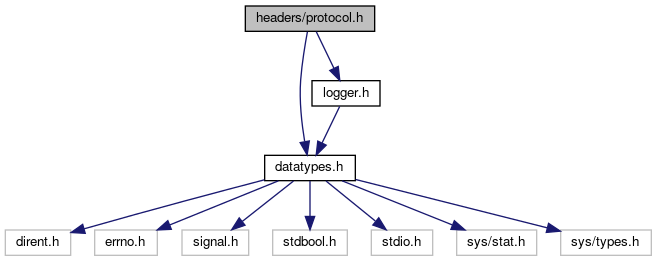
\includegraphics[width=350pt]{protocol_8h__incl}
\end{center}
\end{figure}
This graph shows which files directly or indirectly include this file\+:\nopagebreak
\begin{figure}[H]
\begin{center}
\leavevmode
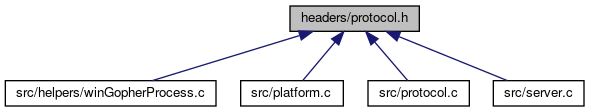
\includegraphics[width=338pt]{protocol_8h__dep__incl}
\end{center}
\end{figure}
\subsection*{Functions}
\begin{DoxyCompactItemize}
\item 
int \hyperlink{protocol_8h_a733e68cc8d5f947c30d0ca51e1b76d9b}{gopher} (socket\+\_\+t sock, int port, const \hyperlink{structlogger__t}{logger\+\_\+t} $\ast$p\+Logger)
\end{DoxyCompactItemize}


\subsection{Detailed Description}
Executes the gopher protocol for a client. 

\subsection{Function Documentation}
\mbox{\Hypertarget{protocol_8h_a733e68cc8d5f947c30d0ca51e1b76d9b}\label{protocol_8h_a733e68cc8d5f947c30d0ca51e1b76d9b}} 
\index{protocol.\+h@{protocol.\+h}!gopher@{gopher}}
\index{gopher@{gopher}!protocol.\+h@{protocol.\+h}}
\subsubsection{\texorpdfstring{gopher()}{gopher()}}
{\footnotesize\ttfamily int gopher (\begin{DoxyParamCaption}\item[{socket\+\_\+t}]{sock,  }\item[{int}]{port,  }\item[{const \hyperlink{structlogger__t}{logger\+\_\+t} $\ast$}]{p\+Logger }\end{DoxyParamCaption})}

Executes the gopher protocol. Receives a selector and performs \hyperlink{protocol_8c_ab628d8ba2c399efb50f6133a3e860c3b}{validate\+Input()} and \hyperlink{protocol_8c_a891da6c8490e699fdf4c10e1275dcf3c}{normalize\+Path()}. If the selector points to a directory, calls \hyperlink{protocol_8c_a57c2a0511da777c6dbcd9f8684308576}{send\+Dir()}. Else, a \hyperlink{structfile__mapping__t}{file\+\_\+mapping\+\_\+t} is created using \hyperlink{platform_8h_a257d48e91fab744f0f71ad79f5acfef2}{get\+File\+Map()} and is sent to the client using \hyperlink{protocol_8c_ae2ef8fc6326f2f545caffbbf8eca0795}{send\+File()}. \begin{DoxyReturn}{Returns}
G\+O\+P\+H\+E\+R\+\_\+\+S\+U\+C\+C\+E\+SS or G\+O\+P\+H\+E\+R\+\_\+\+F\+A\+I\+L\+U\+RE. 
\end{DoxyReturn}

\hypertarget{server_8h}{}\section{headers/server.h File Reference}
\label{server_8h}\index{headers/server.\+h@{headers/server.\+h}}
{\ttfamily \#include $<$netinet/in.\+h$>$}\newline
{\ttfamily \#include $<$stdbool.\+h$>$}\newline
{\ttfamily \#include \char`\"{}datatypes.\+h\char`\"{}}\newline
{\ttfamily \#include \char`\"{}logger.\+h\char`\"{}}\newline
Include dependency graph for server.\+h\+:\nopagebreak
\begin{figure}[H]
\begin{center}
\leavevmode
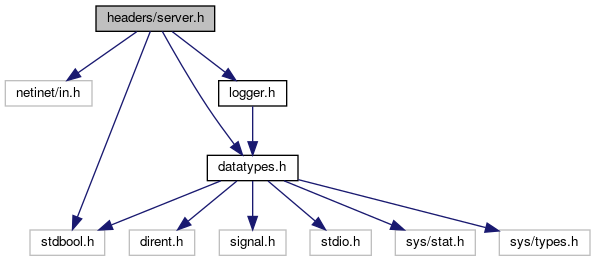
\includegraphics[width=350pt]{server_8h__incl}
\end{center}
\end{figure}
This graph shows which files directly or indirectly include this file\+:\nopagebreak
\begin{figure}[H]
\begin{center}
\leavevmode
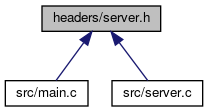
\includegraphics[width=169pt]{server_8h__dep__incl}
\end{center}
\end{figure}
\subsection*{Data Structures}
\begin{DoxyCompactItemize}
\item 
struct \hyperlink{structserver__t}{server\+\_\+t}
\item 
struct \hyperlink{structserver__thread__args__t}{server\+\_\+thread\+\_\+args\+\_\+t}
\end{DoxyCompactItemize}
\subsection*{Functions}
\begin{DoxyCompactItemize}
\item 
int \hyperlink{server_8h_ac6c8652ff4c2d582d1793c14bafd5756}{init\+Wsa} ()
\item 
int \hyperlink{server_8h_a6db637a291288a25af4d89d9f0f3ab31}{install\+Default\+Sig\+Handlers} ()
\item 
int \hyperlink{server_8h_a4c40ae864a752c34a4f237a9445db202}{prepare\+Socket} (\hyperlink{structserver__t}{server\+\_\+t} $\ast$p\+Server, int flags)
\item 
void \hyperlink{server_8h_a2cda6ac8456a82040d05596906d66acc}{default\+Config} (\hyperlink{structserver__t}{server\+\_\+t} $\ast$p\+Server, int which)
\item 
int \hyperlink{server_8h_a2e07cc3959eab913ab4c894bc6c8395d}{read\+Config} (\hyperlink{structserver__t}{server\+\_\+t} $\ast$p\+Server, int which)
\item 
int \hyperlink{server_8h_a533c9a4292e9d1106ff7c54fbf75090a}{run\+Server} (\hyperlink{structserver__t}{server\+\_\+t} $\ast$p\+Server, \hyperlink{structlogger__t}{logger\+\_\+t} $\ast$p\+Logger)
\end{DoxyCompactItemize}


\subsection{Detailed Description}
Functions to manage the main server. 

\subsection{Function Documentation}
\mbox{\Hypertarget{server_8h_a2cda6ac8456a82040d05596906d66acc}\label{server_8h_a2cda6ac8456a82040d05596906d66acc}} 
\index{server.\+h@{server.\+h}!default\+Config@{default\+Config}}
\index{default\+Config@{default\+Config}!server.\+h@{server.\+h}}
\subsubsection{\texorpdfstring{default\+Config()}{defaultConfig()}}
{\footnotesize\ttfamily void default\+Config (\begin{DoxyParamCaption}\item[{\hyperlink{structserver__t}{server\+\_\+t} $\ast$}]{p\+Server,  }\item[{int}]{which }\end{DoxyParamCaption})}

Sets the default options. 
\begin{DoxyParams}{Parameters}
{\em p\+Server} & The \hyperlink{structserver__t}{server\+\_\+t} struct representing the server where the options will be stored. \\
\hline
{\em which} & A flag stating the option to default. Can be R\+E\+A\+D\+\_\+\+P\+O\+RT, R\+E\+A\+D\+\_\+\+M\+U\+L\+T\+I\+P\+R\+O\+C\+E\+SS or both or-\/ed. \\
\hline
\end{DoxyParams}
\mbox{\Hypertarget{server_8h_ac6c8652ff4c2d582d1793c14bafd5756}\label{server_8h_ac6c8652ff4c2d582d1793c14bafd5756}} 
\index{server.\+h@{server.\+h}!init\+Wsa@{init\+Wsa}}
\index{init\+Wsa@{init\+Wsa}!server.\+h@{server.\+h}}
\subsubsection{\texorpdfstring{init\+Wsa()}{initWsa()}}
{\footnotesize\ttfamily int init\+Wsa (\begin{DoxyParamCaption}{ }\end{DoxyParamCaption})}

Initializes a \hyperlink{structserver__t}{server\+\_\+t} struct for further usage. 
\begin{DoxyParams}{Parameters}
{\em p\+Server} & A pointer to the \hyperlink{structserver__t}{server\+\_\+t} struct to initialize. \\
\hline
\end{DoxyParams}
\begin{DoxyReturn}{Returns}
S\+E\+R\+V\+E\+R\+\_\+\+S\+U\+C\+C\+E\+SS or S\+E\+R\+V\+E\+R\+\_\+\+F\+A\+I\+L\+U\+RE. 
\end{DoxyReturn}
\mbox{\Hypertarget{server_8h_a6db637a291288a25af4d89d9f0f3ab31}\label{server_8h_a6db637a291288a25af4d89d9f0f3ab31}} 
\index{server.\+h@{server.\+h}!install\+Default\+Sig\+Handlers@{install\+Default\+Sig\+Handlers}}
\index{install\+Default\+Sig\+Handlers@{install\+Default\+Sig\+Handlers}!server.\+h@{server.\+h}}
\subsubsection{\texorpdfstring{install\+Default\+Sig\+Handlers()}{installDefaultSigHandlers()}}
{\footnotesize\ttfamily int install\+Default\+Sig\+Handlers (\begin{DoxyParamCaption}{ }\end{DoxyParamCaption})}

Installs the default signal handlers for the main process. On Windows, C\+T\+R\+L\+\_\+C interrupts the server and C\+T\+R\+L\+\_\+\+B\+R\+E\+AK requests a configuration update. On Linux, S\+I\+G\+I\+NT interrupts the server and S\+I\+G\+H\+UP requests a configuration update. \begin{DoxyReturn}{Returns}
S\+E\+R\+V\+E\+R\+\_\+\+S\+U\+C\+C\+E\+SS or S\+E\+R\+V\+E\+R\+\_\+\+F\+A\+I\+L\+U\+RE. 
\end{DoxyReturn}
\mbox{\Hypertarget{server_8h_a4c40ae864a752c34a4f237a9445db202}\label{server_8h_a4c40ae864a752c34a4f237a9445db202}} 
\index{server.\+h@{server.\+h}!prepare\+Socket@{prepare\+Socket}}
\index{prepare\+Socket@{prepare\+Socket}!server.\+h@{server.\+h}}
\subsubsection{\texorpdfstring{prepare\+Socket()}{prepareSocket()}}
{\footnotesize\ttfamily int prepare\+Socket (\begin{DoxyParamCaption}\item[{\hyperlink{structserver__t}{server\+\_\+t} $\ast$}]{p\+Server,  }\item[{int}]{flags }\end{DoxyParamCaption})}

Initializes a server socket and sets it to listening. 
\begin{DoxyParams}{Parameters}
{\em p\+Server} & The \hyperlink{structserver__t}{server\+\_\+t} struct representing the server \\
\hline
{\em flags} & Can be S\+E\+R\+V\+E\+R\+\_\+\+U\+P\+D\+A\+TE if a change of port was requested, or S\+E\+R\+V\+E\+R\+\_\+\+I\+N\+IT if the socket must be initialized from scratch. \\
\hline
\end{DoxyParams}
\begin{DoxyReturn}{Returns}
S\+E\+R\+V\+E\+R\+\_\+\+S\+U\+C\+C\+E\+SS or S\+E\+R\+V\+E\+R\+\_\+\+F\+A\+I\+L\+U\+RE. 
\end{DoxyReturn}
\mbox{\Hypertarget{server_8h_a2e07cc3959eab913ab4c894bc6c8395d}\label{server_8h_a2e07cc3959eab913ab4c894bc6c8395d}} 
\index{server.\+h@{server.\+h}!read\+Config@{read\+Config}}
\index{read\+Config@{read\+Config}!server.\+h@{server.\+h}}
\subsubsection{\texorpdfstring{read\+Config()}{readConfig()}}
{\footnotesize\ttfamily int read\+Config (\begin{DoxyParamCaption}\item[{\hyperlink{structserver__t}{server\+\_\+t} $\ast$}]{p\+Server,  }\item[{int}]{which }\end{DoxyParamCaption})}

Reads the options from a configuration file. 
\begin{DoxyParams}{Parameters}
{\em p\+Server} & The \hyperlink{structserver__t}{server\+\_\+t} struct representing the server where the options will be stored. \\
\hline
{\em which} & A flag stating the option to default. Can be R\+E\+A\+D\+\_\+\+P\+O\+RT, R\+E\+A\+D\+\_\+\+M\+U\+L\+T\+I\+P\+R\+O\+C\+E\+SS or both or-\/ed. \\
\hline
\end{DoxyParams}
\begin{DoxyReturn}{Returns}
S\+E\+R\+V\+E\+R\+\_\+\+S\+U\+C\+C\+E\+SS or S\+E\+R\+V\+E\+R\+\_\+\+F\+A\+I\+L\+U\+RE. 
\end{DoxyReturn}
\mbox{\Hypertarget{server_8h_a533c9a4292e9d1106ff7c54fbf75090a}\label{server_8h_a533c9a4292e9d1106ff7c54fbf75090a}} 
\index{server.\+h@{server.\+h}!run\+Server@{run\+Server}}
\index{run\+Server@{run\+Server}!server.\+h@{server.\+h}}
\subsubsection{\texorpdfstring{run\+Server()}{runServer()}}
{\footnotesize\ttfamily int run\+Server (\begin{DoxyParamCaption}\item[{\hyperlink{structserver__t}{server\+\_\+t} $\ast$}]{p\+Server,  }\item[{\hyperlink{structlogger__t}{logger\+\_\+t} $\ast$}]{p\+Logger }\end{DoxyParamCaption})}

Starts a gopher server. 
\begin{DoxyParams}{Parameters}
{\em p\+Server} & A \hyperlink{structserver__t}{server\+\_\+t} struct representing the server to run. \\
\hline
{\em p\+Logger} & A \hyperlink{structlogger__t}{logger\+\_\+t} struct representing the transfer logging process (can be N\+U\+LL). \\
\hline
\end{DoxyParams}
\begin{DoxyReturn}{Returns}
S\+E\+R\+V\+E\+R\+\_\+\+S\+U\+C\+C\+E\+SS if the server is terminated by the user, S\+E\+R\+V\+E\+R\+\_\+\+F\+A\+I\+L\+U\+RE otherwise. 
\end{DoxyReturn}

\hypertarget{wingetopt_8h}{}\section{headers/wingetopt.h File Reference}
\label{wingetopt_8h}\index{headers/wingetopt.\+h@{headers/wingetopt.\+h}}
\subsection*{Macros}
\begin{DoxyCompactItemize}
\item 
\#define \hyperlink{wingetopt_8h_aa3a5661db8614a3b57a1c1d355babd12}{\+\_\+\+W\+I\+N\+G\+E\+T\+O\+P\+T\+\_\+\+H\+\_\+}
\end{DoxyCompactItemize}
\subsection*{Functions}
\begin{DoxyCompactItemize}
\item 
int \hyperlink{wingetopt_8h_ade3a0f38fad659ab1b670b3a28c328ea}{getopt} (int argc, char $\ast$$\ast$argv, char $\ast$opts)
\end{DoxyCompactItemize}
\subsection*{Variables}
\begin{DoxyCompactItemize}
\item 
int \hyperlink{wingetopt_8h_ae30f05ee1e2e5652f174a35c7875d25e}{opterr}
\item 
int \hyperlink{wingetopt_8h_ad5e1c16213bbee2d5e8cc363309f418c}{optind}
\item 
int \hyperlink{wingetopt_8h_a475b8db98445da73e5f62a1ef6324b95}{optopt}
\item 
char $\ast$ \hyperlink{wingetopt_8h_adb50a0eab9fed92fc3bfc7dfa4f2c410}{optarg}
\end{DoxyCompactItemize}


\subsection{Macro Definition Documentation}
\mbox{\Hypertarget{wingetopt_8h_aa3a5661db8614a3b57a1c1d355babd12}\label{wingetopt_8h_aa3a5661db8614a3b57a1c1d355babd12}} 
\index{wingetopt.\+h@{wingetopt.\+h}!\+\_\+\+W\+I\+N\+G\+E\+T\+O\+P\+T\+\_\+\+H\+\_\+@{\+\_\+\+W\+I\+N\+G\+E\+T\+O\+P\+T\+\_\+\+H\+\_\+}}
\index{\+\_\+\+W\+I\+N\+G\+E\+T\+O\+P\+T\+\_\+\+H\+\_\+@{\+\_\+\+W\+I\+N\+G\+E\+T\+O\+P\+T\+\_\+\+H\+\_\+}!wingetopt.\+h@{wingetopt.\+h}}
\subsubsection{\texorpdfstring{\+\_\+\+W\+I\+N\+G\+E\+T\+O\+P\+T\+\_\+\+H\+\_\+}{\_WINGETOPT\_H\_}}
{\footnotesize\ttfamily \#define \+\_\+\+W\+I\+N\+G\+E\+T\+O\+P\+T\+\_\+\+H\+\_\+}



\subsection{Function Documentation}
\mbox{\Hypertarget{wingetopt_8h_ade3a0f38fad659ab1b670b3a28c328ea}\label{wingetopt_8h_ade3a0f38fad659ab1b670b3a28c328ea}} 
\index{wingetopt.\+h@{wingetopt.\+h}!getopt@{getopt}}
\index{getopt@{getopt}!wingetopt.\+h@{wingetopt.\+h}}
\subsubsection{\texorpdfstring{getopt()}{getopt()}}
{\footnotesize\ttfamily int getopt (\begin{DoxyParamCaption}\item[{int}]{argc,  }\item[{char $\ast$$\ast$}]{argv,  }\item[{char $\ast$}]{opts }\end{DoxyParamCaption})}



\subsection{Variable Documentation}
\mbox{\Hypertarget{wingetopt_8h_adb50a0eab9fed92fc3bfc7dfa4f2c410}\label{wingetopt_8h_adb50a0eab9fed92fc3bfc7dfa4f2c410}} 
\index{wingetopt.\+h@{wingetopt.\+h}!optarg@{optarg}}
\index{optarg@{optarg}!wingetopt.\+h@{wingetopt.\+h}}
\subsubsection{\texorpdfstring{optarg}{optarg}}
{\footnotesize\ttfamily char$\ast$ optarg}

\mbox{\Hypertarget{wingetopt_8h_ae30f05ee1e2e5652f174a35c7875d25e}\label{wingetopt_8h_ae30f05ee1e2e5652f174a35c7875d25e}} 
\index{wingetopt.\+h@{wingetopt.\+h}!opterr@{opterr}}
\index{opterr@{opterr}!wingetopt.\+h@{wingetopt.\+h}}
\subsubsection{\texorpdfstring{opterr}{opterr}}
{\footnotesize\ttfamily int opterr}

\mbox{\Hypertarget{wingetopt_8h_ad5e1c16213bbee2d5e8cc363309f418c}\label{wingetopt_8h_ad5e1c16213bbee2d5e8cc363309f418c}} 
\index{wingetopt.\+h@{wingetopt.\+h}!optind@{optind}}
\index{optind@{optind}!wingetopt.\+h@{wingetopt.\+h}}
\subsubsection{\texorpdfstring{optind}{optind}}
{\footnotesize\ttfamily int optind}

\mbox{\Hypertarget{wingetopt_8h_a475b8db98445da73e5f62a1ef6324b95}\label{wingetopt_8h_a475b8db98445da73e5f62a1ef6324b95}} 
\index{wingetopt.\+h@{wingetopt.\+h}!optopt@{optopt}}
\index{optopt@{optopt}!wingetopt.\+h@{wingetopt.\+h}}
\subsubsection{\texorpdfstring{optopt}{optopt}}
{\footnotesize\ttfamily int optopt}


%--- End generated contents ---

% Index
\backmatter
\newpage
\phantomsection
\clearemptydoublepage
\addcontentsline{toc}{chapter}{Index}
\printindex

\end{document}
